\documentclass[11pt,a4paper]{article}

\usepackage{chngcntr}
\usepackage{subcaption}

\counterwithin{figure}{section}
\counterwithin{table}{section}
\usepackage{xcolor}
\usepackage{listings}

\definecolor{codegray}{gray}{0.95}
\definecolor{commentgreen}{rgb}{0.0,0.45,0.0}
\definecolor{keywordblue}{rgb}{0.0,0.2,0.6}

\lstdefinestyle{pythonappendix}{
    language=Python,
    basicstyle=\ttfamily\scriptsize,
    backgroundcolor=\color{codegray},
    keywordstyle=\color{keywordblue}\bfseries,
    commentstyle=\color{commentgreen},
    stringstyle=\color{black},
    numbers=left,
    numberstyle=\tiny,
    stepnumber=1,
    numbersep=6pt,
    frame=single,
    breaklines=true,
    breakatwhitespace=false,
    showstringspaces=false,
    tabsize=4,
    captionpos=b
}
\usepackage{algorithm}
\usepackage{algpseudocode}
\usepackage[ruled,vlined,linesnumbered]{algorithm2e}
\SetAlgoCaptionSeparator{:}

\lstset{
    basicstyle=\ttfamily\small,
    breaklines=true,
    frame=single,
    columns=fullflexible,
    keepspaces=true,
    showstringspaces=false,
    language=Python
}
\usepackage[T1]{fontenc}
\usepackage[utf8]{inputenc}
\usepackage{lmodern}
\usepackage[a4paper, margin=2.5cm]{geometry}
\usepackage{setspace}
\usepackage{amsmath, amssymb, amsthm}
\usepackage{graphicx}
\usepackage{booktabs}
\usepackage{array}
\usepackage{float}
\usepackage[hidelinks]{hyperref}
\newcommand{\hcite}[2]{\hyperlink{#1}{#2}}
\newcommand{\hcite}[2]{\hyperlink{#1}{#2}}
\usepackage{appendix}
\usepackage[font=small,labelfont=bf]{caption}
\usepackage{enumitem}
\usepackage{xurl}
\usepackage[hyphens]{url}
\hypersetup{breaklinks=true}
\Urlmuskip=0mu plus 1mu
\setlength{\emergencystretch}{3em}
\onehalfspacing
\setlength{\parindent}{0pt}
\setlength{\parskip}{0.8em}
%\setcounter{tocdepth}{1}

\title{Modelling Public Transport Accessibility and Commuting Inequality: A Generalised Cost Approach for Cardiff University Staff}
\author{Eve Williamson}
\date{2026}

\begin{document}


\begin{titlepage}
\centering

\vspace*{2.5cm}

{\Large\bfseries Modelling Public Transport Accessibility and Commuting Inequality:\par}
\vspace{0.25cm}
{\Large\bfseries A Generalised Cost Approach for Cardiff University Staff\par}

\vspace{2cm}

{\large Eve Williamson\par}
\vspace{0.4cm}


\vspace{1.5cm}

{\large Financial Mathematics\par}
\vspace{0.25cm}
{\large Department of Mathematics\par}
\vspace{0.25cm}
{\large Cardiff University\par}

\vspace{1.5cm}

{\large Supervisor: Professor Jon Gillard\par}

\vfill

{\large 2026\par}

\end{titlepage}

\section*{Executive Summary}


This project develops a mathematical accessibility cost index to quantify
the public transport burden of commuting to Cardiff University campuses from
different LSOAs across Cardiff. The study combines GIS-based spatial analysis,
public transport route modelling, and statistical analysis to examine whether
higher transport cost is associated with deprivation and with greater reliance
on the car. By moving beyond descriptive mode-share analysis, the project
formalises commuting burden using weighted travel time, temporal variability,
monetary fare, and an explicit treatment of inaccessible areas.
The results show that Cardiff-based staff are disproportionately concentrated in less deprived areas, particularly in higher WIMD deciles (8-10). Public transport accessibility varies substantially across Cardiff and differs between campuses, with Heath Park exhibiting higher generalised accessibility costs than Cathays. The accessibility cost index is positively associated with single-occupancy car (SOC) driving frequency, although the relationship is modest and weakens when deprivation is controlled for. The index outperforms simpler service-based measures such as bus stop counts and departures, supporting the use of route-based generalised cost measures for analysing commuting accessibility. The findings suggest that sustainable travel policy should focus on reducing actual journey burden, particularly for Heath Park and for staff in more deprived areas.

\newpage
\tableofcontents
\newpage


\section{Introduction}

\subsection{Background and Motivation}

The 2024 Cardiff University Staff Travel Survey, a key dataset in this research, was conducted in support of the University’s Our Future, Together strategy and its five‑year Travel Plan. These initiatives aim to reduce transport‑related carbon emissions while improving access to sustainable travel options, contributing to the University’s wider ambition of achieving net‑zero scope 1 and 2 emissions by 2030 and scope 3 emissions by 2050 (\hcite{cardiff2025}{Cardiff University, 2025}).
Initial GIS and statistical analysis showed that, despite the encouragement of sustainable travel, its feasibility varies across locations. Some commuters experience longer journey times, poorer service availability, and a higher overall travel burden; all of which affect accessibility to campus.
In the context of Cardiff University, this is particularly relevant as accessibility varies between campuses. Heath is not only a teaching campus but also the location of the University Hospital, while Cathays is more centrally located and contains a larger concentration of academic facilities. In higher education, staff commuting is particularly important because it contributes to carbon emissions, congestion, and local air pollution, while also affecting access to work and campus facilities.
To address this, the study constructs a route‑based public transport accessibility cost index using a generalised cost framework. The project examines how this cost index varies across space and whether it is associated with commuting behaviour and deprivation. Using Cardiff University staff travel survey data, Welsh Index of Multiple Deprivation data and route‑based transport modelling, it investigates whether higher transport costs are linked to greater car use and whether staff in more deprived areas face different commuting conditions. Accessibility is therefore treated as both a spatial and social issue, measured quantitatively to understand transport inequality among Cardiff University staff.


\subsection{Research Problem}

This dissertation examines how deprivation, transport accessibility, distance, and commuting costs interact to influence staff travel behaviour, with a particular emphasis on single-occupancy car use. The core research question investigates whether staff residing in more deprived or less accessible areas experience systematically poorer access to Cardiff University campuses, and consequently adopt different commuting patterns.

To address this, the study constructs a mathematically defined accessibility cost index tailored to commuting to Cardiff University and applies statistical methods to examine its relationship with both deprivation and mode of travel. In addition, it evaluates whether a time-based generalised cost measure offers a more accurate representation of accessibility compared to simpler proxies, such as bus stop density.


\subsection{Research Questions}

The study is guided by the following research questions:

\begin{enumerate}
    \item How can public transport accessibility to Cardiff University campuses be quantified using a route-based generalised cost index?
    \item How does public transport accessibility vary spatially across Cardiff and between Cathays and Heath Park campuses?
    \item What is the relationship between public transport accessibility, area-level deprivation and staff commuting behaviour?
    \item Does the generalised accessibility cost index provide a more informative measure of commuting burden than simpler service-based indicators such as bus stop counts and departures?
\end{enumerate}

\subsection{Structure of the Project}

The dissertation is structured as follows. Section 2 reviews the literature on accessibility, generalised cost, transport inequality, deprivation and commuting behaviour. Section 3 outlines the methodological framework, including survey preparation, GIS integration, public transport routing and statistical analysis. Section 4 presents the construction of the accessibility cost index. Section 5 reports the empirical results, including spatial patterns of deprivation, public transport accessibility, driving behaviour, regression analysis, robustness checks and incentive preferences. Section 6 discusses the findings in relation to the literature, methodological limitations and policy implications. Section 7 concludes by summarising the main findings and identifying directions for future research.
\newpage

\section{Literature Review}

This chapter reviews the literature on accessibility, transport inequality, and commuting behaviour. It first outlines the limitations of conventional accessibility measures before introducing generalised cost as a more comprehensive framework. It then examines how accessibility interacts with social exclusion, deprivation, and mode choice, before situating these themes within the context of Cardiff University. The chapter concludes by identifying a gap in integrating route-level accessibility, deprivation, and observed commuting behaviour.

\subsection{Accessibility and Generalised Cost}

Accessibility is a core concept in transport geography, defined as ``the extent to which land-use and transport systems enable (or constrain) activity participation'' \hcite{geurs2004}{(Geurs and van Wee, 2004)}. \hcite{geurs2004}{Geurs and van Wee (2004)} identify four components of accessibility: land-use (distribution of opportunities), transport (cost of reaching them), temporal factors (time constraints and service availability), and individual characteristics (needs, abilities, and resources). However, traditional measures such as stop density or travel time primarily capture the transport component while neglecting temporal variability and individual constraints. Although widely used due to their simplicity, such measures are theoretically limited.

Proximity-based indicators, such as counting stops or stations within a fixed distance, provide only a partial measure of accessibility as they fail to capture the ease or cost of reaching destinations. \hcite{handy1997}{Handy and Niemeier (1997)} argue that accessibility depends on the ``ease of reaching each destination'' and that generalised transport cost, incorporating both time and monetary cost, is more appropriate than time alone. This limitation has led to the development of more comprehensive measures of accessibility.

Responding to these limitations, transport research developed the concept of generalised cost, which aggregates multiple journey attributes into a single measure of impedance. This framework reflects how individuals make decisions between attributes such as time and cost (\hcite{domencich1975}{Domencich and McFadden, 1975}), consistent with discrete choice theory (\hcite{mcfadden1974}{McFadden, 1974}). Early UK appraisal treated journey components using fixed weightings. Based on work carried out for the then Ministry of Transport, walking and waiting time were typically valued at approximately twice in-vehicle time (IVT), reflecting the higher perceived burden of out-of-vehicle travel (McIntosh and Quarmby, 1970, as cited in \hcite{mackie2003}{Mackie et al., 2003}).

Subsequent work refines these assumptions. \hcite{wardman2004}{Wardman (2004)} estimates walking time at approximately $2\times$ IVT and waiting time at around $2.5\times$ IVT, while more recent European evidence suggests lower values. \hcite{wardman2016}{Wardman, Chintakayala and de Jong (2016)} find walking and waiting time are valued at approximately 45\% and 50\% more than IVT respectively, noting this is ``somewhat less than the factor of two commonly applied''. These findings indicate that, although out-of-vehicle time remains more burdensome, conventional appraisal assumptions may overstate its effect. However, generalised cost remains sensitive to the choice of parameter weightings, which are often context-dependent and may not fully capture individual heterogeneity.

Importantly, these valuations are defined relative to IVT, meaning journey components are expressed within a unified generalised cost framework rather than treated independently.

\begin{table}[H]
\centering
\caption{Evolution of walking and waiting time valuations}
\label{tab:vott}
\begin{tabular}{lccc}
\toprule
\textbf{Period} & \textbf{Walking VOTT} & \textbf{Waiting VOTT} & \textbf{Source} \\
\midrule
1960s & $2.0\times$ IVT & $2.0\times$ IVT & \hcite{mackie2003}{Mackie et al. (2003)} \\
2004  & $\sim 2.0\times$ IVT & $\sim 2.5\times$ IVT & \hcite{wardman2004}{Wardman (2004)} \\
2016  & $1.45\times$ IVT & $1.50\times$ IVT & \hcite{wardman2016}{Wardman et al. (2016)} \\
\bottomrule
\end{tabular}
\caption*{\footnotesize Note: The 1960s values refer to McIntosh and Quarmby's work for the Ministry of Transport, as reported by Mackie et al. (2003).}
\end{table}
Recent research extends this critique by showing that accessibility is not purely spatial or static, but varies over time and across individuals. \hcite{ryan2023}{Ryan, Pereira and Andersson (2023)} show that accessibility is shaped by temporal factors, such as peak versus off-peak time, and by individual constraints including income, car ownership, transport mode availability, and childcare commitments. In addition, static timetable-based measures may overestimate accessibility by failing to account for real-world service disruption (\hcite{liu2022}{Liu, Porr and Miller, 2022}). Measures that exclude these factors may therefore underestimate the burden of public transport accessibility. Accessibility is therefore not only a technical measure of transport systems, but also has clear implications for inequality and social outcomes.

\subsection{Transport Inequality and Social Exclusion}

Transport underpins participation in everyday activities, but access to it is not evenly distributed. \hcite{lucas2012}{Lucas (2012)} identifies transport disadvantage as a barrier to employment, education and healthcare, placing transport policy within a broader social inclusion agenda. \hcite{preston2007}{Preston and Rajé (2007)} extend this argument by showing that social exclusion is not simply a function of low mobility, but of limited access to opportunities. Participation therefore depends on the ability to reach key services and activities, rather than travel itself. This implies that individuals may travel frequently yet still face barriers to participation.

In a UK context, the \hcite{socialexclusion2003}{Social Exclusion Unit (2003)} highlights how these barriers contribute to persistent disadvantage. \hcite{hine2003}{Hine and Grieco (2003)} argue that transport disadvantage is not only spatially clustered but also occurs in dispersed ``scatters'', where exclusion correlates to personal circumstances such as age, disability, or social isolation. This distinction suggests that area-based transport policies may fail to capture all forms of exclusion. In the context of this study, this also implies that aggregate spatial accessibility measures may obscure individual disadvantage.

Altogether, this suggests that transport accessibility cannot be treated as a neutral, purely technical issue. Instead, it reflects a set of structural constraints that shape who can access opportunities and who cannot, with these constraints often reinforcing existing inequalities.

\subsection{Deprivation and Spatial Inequality}

Deprivation provides a way of understanding how these inequalities are distributed across space. The Welsh Index of Multiple Deprivation (WIMD) is the official measure of area-level deprivation in Wales, combining multiple domains to capture socioeconomic disadvantage at LSOA level (\hcite{welshgov2019}{Welsh Government, 2019}). It allows accessibility to be analysed alongside broader structural domains, including income, employment, health, education, access to services, community safety, physical environment and housing.

Evidence suggests that transport constraints are more pronounced in deprived areas, particularly where service provision is limited or declining. \hcite{price2022}{Price, Higgs and Langford (2022)} show that reductions in bus service accessibility during the COVID-19 period disproportionately affected more deprived communities in Wales, reinforcing existing inequalities. As shown in Figure~\ref{fig:wimd_bus_decline}, the largest declines in accessibility occur in the most deprived deciles, highlighting the unequal spatial impact of service reductions. This is reinforced by evidence that 12\% of people in Wales have no access to public transport services in their local area, alongside evidence that low-income households and other vulnerable groups face significant barriers to accessing transport (\hcite{sustrans2022}{Sustrans Cymru, 2022}).

\begin{figure}[H]
\centering
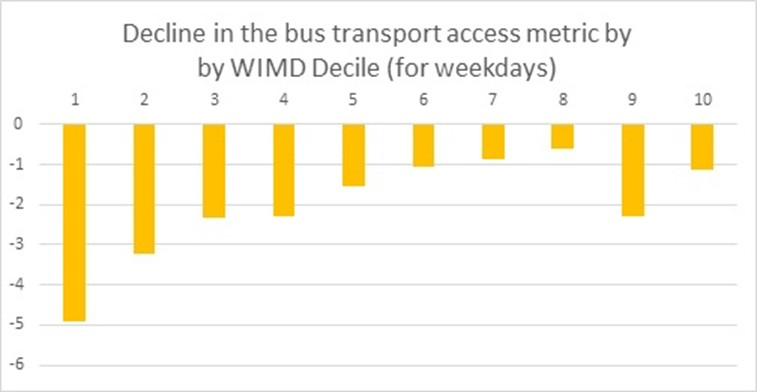
\includegraphics[width=0.8\textwidth]{Prices, Higgs and Langford.jpg}
\caption{Changes in access scores by WIMD 2019 decile, 2019-2021. WIMD decile 1 = most deprived; 10 = least deprived. Source: Price, Higgs and Langford (2022).}
\label{fig:wimd_bus_decline}
\end{figure}

While WIMD 2025 has since been released, WIMD 2019 remains appropriate for this study as it aligns with the temporal context of the dataset and ensures consistency in spatial analysis. Overall, these findings indicate that accessibility constraints are not randomly distributed, but are closely linked to area-level deprivation.

\subsection{Commuting Behaviour and Mode Choice}

Commuting behaviour reflects trade-offs between time and monetary cost. \hcite{vanommeren2006}{Van Ommeren and Dargay (2006)} model commuting speed as a cost-minimising choice, where commuters choose faster travel when the value-of-time savings outweighs the additional monetary cost. Their findings suggest that income affects commuting speed, with higher-income commuters more likely to choose faster, more expensive modes. This is consistent with evidence that ``higher incomes increase the opportunity costs of travel time---thus making faster modes of transport... more attractive'' (\hcite{buehler2011}{Buehler, 2011}). Together, these findings support a generalised cost interpretation of commuting behaviour, where travel decisions reflect both time and financial constraints.

Car availability is a key constraint on mode choice. \hcite{buehler2011}{Buehler (2011)} shows that fewer cars per licensed household member are associated with lower levels of car use. \hcite{scheiner2012}{Scheiner and Holz-Rau (2012)} extend this by demonstrating that in car-deficient households, where there are fewer cars than licensed drivers, access is unevenly allocated; licensed men made 56.6\% of trips by car compared with 36.5\% for licensed women. This suggests that car access is not simply binary, but shaped by competition within households.

Reliability and time variability further influence mode choice. \hcite{bates2001}{Bates et al., 2001} identify reliability as ``a major issue in travel choice'', with travellers often placing greater value on reductions in variability than in average journey time. As a result, commuters may prioritise the predictability of private vehicle travel over the uncertainty of public transport. Commuting patterns are therefore not solely a function of distance, but reflect broader socioeconomic and temporal constraints. This reinforces the relevance of modelling commuting behaviour through a generalised cost framework, where both time and monetary constraints shape observed choices.

\subsection{University and Cardiff Context}

Universities are major trip generators and face increasing pressure to reduce commuting-related emissions. As an anchor institution, Cardiff University integrates sustainable transport into its strategic framework, making staff commuting a relevant policy concern. Its multi-campus structure, contrasting the central Cathays site with the more distant Heath Park site, creates variation in accessibility that supports comparative analysis.

\hcite{betts2025}{Betts and Potoglou, 2025} show that travel behaviour in Cardiff varies by deprivation. Private vehicle use in 2018-19 reached 71.9\% in the least deprived group, compared with 50.6\% in the most deprived. Active commuting also increased overall, rising from 24.2\% to 33.3\% between 2018-19 and 2019-20, although this increase was not uniform; middle deprivation areas experienced a larger rise, from 28.2\% to 43.9\% (Table A2). These patterns indicate that commuting inequality is a current concern for the city, reflecting underlying socioeconomic differences associated with deprivation.

By applying a route-based generalised cost framework to Cardiff University staff, this study connects theoretical models of accessibility with the practical realities of commuting in an uneven urban transport network.

\subsection{Synthesis}

While accessibility is widely recognised as multidimensional, it is often simplified in practice through static spatial measures. Generalised cost offers a more robust approach by capturing the overall burden of travel, rather than relying on distance or time alone. However, the literature tends to treat these theoretical developments separately from the socioeconomic realities of commuting behaviour, with limited integration between accessibility modelling and inequality analysis.

This creates a clear empirical gap, particularly in university contexts, where route-level variation, value-of-time assumptions and spatial inequality are rarely examined together. Given its emphasis on sustainable transport and modal shift, alongside its multi-campus structure, Cardiff University provides a useful setting in which these relationships can be explored. The variation in accessibility across sites further strengthens its relevance for analysing how transport burden differs across populations.

This study addresses this gap by applying a route-based generalised cost framework to staff travel, allowing accessibility to be examined alongside deprivation and observed commuting outcomes.

\section{Methodology}
\subsection{Research Design}

This study employs a quantitative spatial analytical framework to investigate the relationship between area-level deprivation, public transport accessibility and the commuting behaviour of staff at Cardiff University. The methodology integrates survey-derived travel data with public transport network data and spatial indicators to examine how commuting accessibility varies across Cardiff and how this relates to observed travel behaviour.

The research uses four primary data sources: the 2024 Cardiff University Staff Travel Survey, the 2019 Welsh Index of Multiple Deprivation (WIMD), General Transit Feed Specification (GTFS) data from Cardiff Bus, and time-dependent travel data extracted using the Google Routes API. To ensure spatial consistency, these datasets are integrated using Lower Super Output Areas (LSOAs) as the primary unit of analysis. LSOAs are a standardised UK statistical geography representing approximately 1,500 residents. This common spatial framework enables the joint analysis of staff home locations, area-level deprivation and public transport accessibility within a unified dataset.

The methodology is structured in three core stages. First, the staff travel survey data are processed to characterise baseline commuting patterns, with modal choice and driving frequency used as key outcome variables. Second, GIS-based spatial joining techniques are used to link staff residential postcodes to their corresponding LSOAs, allowing deprivation measures and transport infrastructure data to be integrated. Third, a generalised public transport accessibility cost index is constructed to quantify accessibility at the LSOA level. This index incorporates journey time, monetary cost and temporal variability, with journey components weighted to reflect the relative burden of walking, in-vehicle travel, waiting and interchange.

Public transport accessibility is quantified using time-dependent journey data obtained from the Google Routes API. Journeys are modelled from Cardiff bus stops to the two main campus destinations, Cathays and Heath, under public transport mode and across multiple weekday departure periods. This allows temporal variation in journey times to be captured. Route outputs are decomposed into walking, in-vehicle public transport and residual transfer-related components, allowing accessibility to be represented as a generalised cost rather than a simple measure of proximity or service availability.

Finally, statistical and spatial analysis is used to evaluate relationships between deprivation, accessibility and commuting behaviour. This includes testing for differences in driving frequency across WIMD deprivation deciles and assessing the association between the generalised accessibility cost index and observed travel choices. This methodological design moves beyond proximity-based indicators by measuring the actual burden of reaching campus by public transport, providing a more realistic assessment of commuting accessibility across Cardiff.

\subsection{Staff Travel Survey and Cleaning}

\subsubsection{Survey Design and Response Rate}

The 2024 Staff Travel Survey gathered information on commuting behaviours, workplace destinations and barriers to sustainable travel. Staff provided details on travel mode, reasons for mode choice and home postcode to enable statistical and spatial analysis.

A total of 1,587 responses were received, with 1,509 of these including useable responses. Reasons for excluding participants ($n = 78$) included missing or invalid postcodes, missing campus/building data and unlisted residence buildings without campus information.

With 7,760 staff employed at the University during the same time period of the survey conduction (\hcite{hesa2023}{HESA, 2023}), the eligible response rate was 19.4\% (Table~\ref{tab:response_rate}).

\begin{table}[H]
\centering
\caption{Staff survey responses and response rate}
\label{tab:response_rate}
\begin{tabular}{lccc}
\toprule
\textbf{Group} & \textbf{Count} & \textbf{Eligible Count} & \textbf{Eligible Response Rate} \\
\midrule
Staff & 1587 & 1509 & 19.4\% \\
\bottomrule
\end{tabular}
\end{table}

Figure~\ref{fig:campus_distribution} shows the distribution of respondents by primary campus, with the majority based at Cathays Park. This distribution is important for subsequent analysis, as it informs the relative weighting of campus destinations in the accessibility cost index.

\begin{figure}[H]
    \centering
    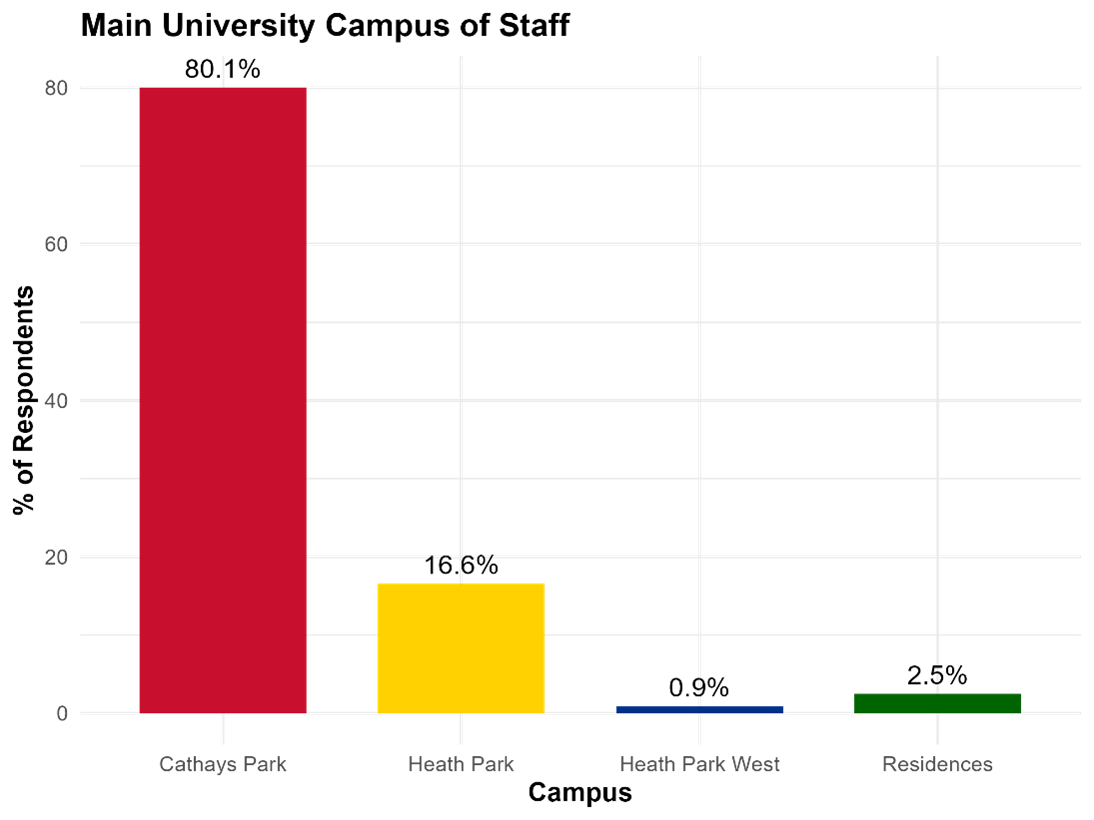
\includegraphics[width=0.72\textwidth]{figures/campus_distribution.png}
    \caption{Distribution of survey responses by primary campus}
    \label{fig:campus_distribution}
\end{figure}

The dominance of Cathays-based respondents indicates that a university-wide accessibility measure should give greater weight to Cathays while still retaining the accessibility burden associated with Heath Park.

\subsubsection{Data Preparation}

The survey dataset underwent a structured preparation process to ensure consistency and suitability for spatial and econometric analysis. Data were processed in R (version 4.5.1), including standardisation of column names and removal of non-essential metadata. Core variables, particularly residential postcodes, campus affiliation, and workplace location, were validated and cleaned. Postcode entries were systematically reviewed using frequency tables and sorting checks to identify inconsistencies and anomalies, with formatting standardised prior to spatial implementation. Records with missing, invalid, or non-geocodable postcodes were excluded, and the cleaned distribution was rechecked to confirm consistency, resulting in a final sample of 1,509 respondents.

Categorical variables, including college and school affiliations, contained substantial variation in naming conventions and were harmonised using manual recoding procedures. Equivalent entries were grouped into consistent categories through string matching and validation checks. The resulting classifications were verified using frequency tables to ensure that equivalent responses had been correctly consolidated.

Free-text responses were standardised and categorised into thematic groupings using an iterative approach combining keyword-based qualitative classification and manual review. NVivo was used to generate word frequency outputs, supporting the identification of recurring themes and validating the consistency of coding decisions.

Additional validation steps were undertaken to identify anomalous values within key variables, including implausible commute distances. These were cross-checked against postcode data and either corrected or recoded as missing values where appropriate. Derived variables were then constructed, including grouped travel modes, commute distance bands, and adjusted driving frequency measures. Driving frequency was corrected for reported work-from-home patterns and non-working days, and summary statistics were reviewed to confirm that transformations produced plausible and internally consistent results.



\subsection{Spatial analysis and GIS integration}

Spatial analysis was conducted using ArcGIS to integrate survey data with geographic and transport datasets within a consistent analytical framework. All spatial data were projected to the British National Grid (OSGB 1936 / EPSG:27700) to ensure consistent measurement of area and distance. The Welsh Index of Multiple Deprivation (WIMD, 2019) was imported at the LSOA level, with deprivation measured using ranks (see Figure~\ref{fig:wimd_choropleth}) and percentiles. Cardiff's administrative boundary was used to define the study area, and all datasets were clipped accordingly to ensure spatial consistency. 

\begin{figure}[H]
    \centering
    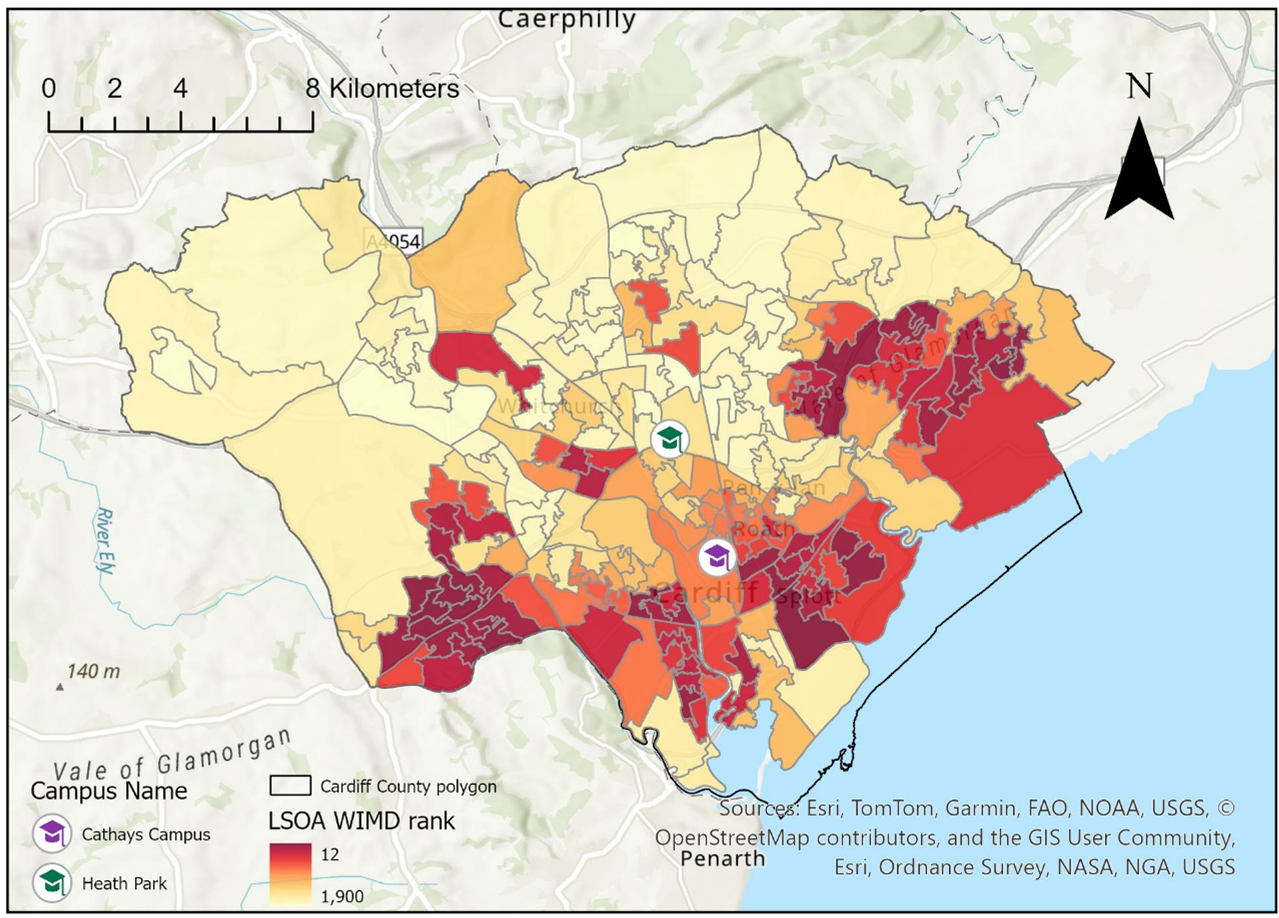
\includegraphics[width=0.85\textwidth]{figures/wimd_choropleth_cardiff.png}
    \caption{Welsh Index of Multiple Deprivation choropleth (Cardiff)}
    \label{fig:wimd_choropleth}
\end{figure}

Figure~\ref{fig:wimd_choropleth} shows the spatial distribution of deprivation alongside the locations of Cathays Campus and Heath Park, which form the primary destinations for staff commuting.

Staff residential locations were geocoded from postcode data and spatially joined to LSOA polygons, linking each respondent to an area-level deprivation measure. Following spatial filtering, 840 respondents were located within the Cardiff boundary and successfully matched to LSOAs, representing approximately 10.8\% of the university workforce ($n = 7,760$). While this provides a substantial spatial sample, the analysis is restricted to Cardiff-based staff and may be subject to spatial self-selection bias.

Public transport infrastructure was incorporated using General Transit Feed Specification (GTFS) data for Cardiff Bus. After clipping to the Cardiff boundary, approximately 2,028 bus stop records were identified. As GTFS data include multiple entries for the same physical location (e.g. by route or direction), this measure represents service-weighted stop counts rather than 974 unique stop locations, capturing the intensity of public transport provision within each LSOA. Bus stops were spatially joined to LSOAs to derive area-level measures of service provision. LSOA polygon areas were calculated in square kilometres using GIS geometry tools and summed to confirm the spatial extent of the Cardiff study area, which is approximately 140 km\textsuperscript{2} (\hcite{means2025}{Means, 2025}). This allowed consistent comparison across areas of different sizes.

In addition to data integration, GIS was used to visualise and interpret accessibility outputs derived from the routing analysis. Route geometries generated from the Google Routes API were converted into GeoJSON format and imported into ArcGIS, allowing journey paths and modal segments to be mapped. Time-based accessibility surfaces were constructed using time-budget mapping techniques, producing isochrone-style representations of reachable areas around campus locations under public transport conditions. These outputs enabled direct spatial comparison of accessibility between the Cathays and Heath sites and supported interpretation of the accessibility cost index. Final map layouts and web maps were exported to present results in a clear spatial format.

All spatial outputs were exported from ArcGIS and integrated into R for final analysis, ensuring that deprivation, infrastructure and accessibility variables were consistently aligned at the LSOA level prior to econometric modelling.

\subsection{Public transport routing and API data}

Traditional accessibility measures based on proximity or stop density were not adopted because they do not capture the time, cost, temporal variability, or structure of real journeys. Instead, public transport accessibility was modelled using route-based travel times generated in Python using the Google Routes API. Alternative approaches, including OpenRouteService and GTFS-based network construction, were initially explored; however, these were limited in their ability to produce time-dependent public transport journeys with full modal decomposition. The Google Routes API was therefore selected, as it provides dynamic transit routing with step-level outputs, including walking stages, modal breakdown, transfer structure and route geometry. The core Python implementation used to generate the route-level CSV outputs is provided in Appendix~\ref{app:computational_implementation}.

\subsubsection{Origin and destination specification}

The origin network was constructed from Cardiff Bus GTFS stop data. After clipping to the Cardiff boundary and removing duplicate stop identifiers, 974 unique bus stops were retained. The resulting distribution of feasible route counts across Cardiff LSOAs is reported in Appendix~\ref{app:graphs_stats}, Figure~\ref{fig:route_count_distribution}. Each stop represents a distinct physical access point to the public transport network, ensuring that routing reflects realistic boarding locations rather than duplicated service entries.

Although the routing model later allowed public transport journeys to include rail segments where identified by the Google Routes API, railway stations were not included as separate origin points in the access network. This is because the two campus destinations differ in their relationship to the rail network. Cathays Campus lies within an accessible walking radius of Cathays railway station, whereas the Heath Park campus destination lies outside an equivalent accessible radius from the nearest railway station.

Including railway stations as additional origin points would therefore have introduced an asymmetric campus effect. Cathays would be able to benefit directly from nearby rail access, while Heath would require an additional penalty or adjustment to reflect its lack of comparable station accessibility. Instead, bus stops were used as the consistent origin network for both campuses. Rail was still incorporated within the API route calculation where it formed part of the fastest available public transport journey, allowing the Cathays cost calculation to reflect faster multimodal routes where these were available.

Two fixed destination points were defined to represent Cardiff University’s primary campuses. Cathays Campus was represented by a central coordinate near the Sir Martin Evans building (51.487207, -3.176992), while Heath Park Campus was represented by a central point within the University Hospital of Wales site (51.507156, -3.189855). Using fixed coordinates ensured that all origin stops were evaluated against consistent destination locations.
\subsubsection{API routing workflow and implementation}

The routing workflow was implemented in Python (Spyder) using a structured looping procedure. The script iterated over each origin stop \(i\), each campus destination \(j\), and each departure hour \(h_k\), as summarised in Algorithm~\ref{alg:routing_workflow}. 

\begin{algorithm}[H]
\caption{Routing workflow for public transport accessibility analysis}
\label{alg:routing_workflow}



\KwIn{Origin bus stops \(i\), campus destinations \(j\), departure hours \(h_k\)}
\KwOut{Route journey times and component-level accessibility outputs}

\ForEach{origin stop \(i\)}{
    \ForEach{campus destination \(j\)}{
        \ForEach{departure hour \(h_k\)}{
            Query route\;
            Extract route components\;
            Store outputs\;
        }
    }
}

\end{algorithm}
Algorithm~\ref{alg:routing_workflow} is implemented in Python through loops over origin stops, campus destinations and sampled departure times. The corresponding implementation is shown in Appendix~\ref{app:computational_implementation}, Listings~\ref{lst:origin_campus_loop}-\ref{lst:departure_time_loop}.

For each origin-campus-time combination, the Google Routes Matrix endpoint was used to retrieve total journey time \(T_{i,j}(h_k)\) and distance, conditional on a valid transit route existing. These outputs formed the core time-dependent accessibility dataset.

Where a valid route was returned, a second request to the Compute Routes endpoint extracted detailed step-level journey information, including travel mode, segment duration, transit line identifiers, and encoded route geometry.

This two-stage approach improved efficiency by using the Matrix endpoint for rapid travel-time estimation while limiting detailed route extraction to valid journeys. All outputs were written to structured CSV files for analysis and GeoJSON files for GIS visualisation.

\subsubsection{Departure time sampling and temporal averaging}

To account for temporal variability in public transport performance, each origin-campus pair was evaluated across a set of eight representative weekday departure hours.

The notation used in the routing and API analysis is summarised in Table~\ref{tab:routing_notation}.

\begin{table}[H]
\centering
\small
\caption{Notation used in public transport routing and API analysis}
\label{tab:routing_notation}
\renewcommand{\arraystretch}{1.25}
\begin{tabular}{ll}
\hline
Symbol & Definition \\
\hline
$i$ & Origin bus stop index \\
$j$ & Campus destination index \\
$h_k$ & Departure hour \\
$\mathcal{H}$ & Set of sampled departure hours \\
$K$ & Number of sampled departure hours \\
$T_{i,j}(h_k)$ & Travel time from origin stop $i$ to campus $j$ at departure hour $h_k$ \\
$\bar{T}_{i,j}$ & Mean travel time from origin stop $i$ to campus $j$ across sampled departure hours \\
$w_{i,j}$ & Walking time from origin stop $i$ to campus $j$ \\
$b_{i,j}$ & Bus in-vehicle time from origin stop $i$ to campus $j$ \\
$q_{i,j}$ & Rail in-vehicle time from origin stop $i$ to campus $j$ \\
$o_{i,j}$ & Other transit in-vehicle time from origin stop $i$ to campus $j$ \\
$v_{i,j}$ & Total in-vehicle time from origin stop $i$ to campus $j$ \\
$r_{i,j}$ & Residual waiting/interchange component from origin stop $i$ to campus $j$ \\
\hline
\end{tabular}
\renewcommand{\arraystretch}{1}
\end{table}

Let

\[
\mathcal{H} = \{07{:}00, 08{:}00, 09{:}00, 10{:}00, 16{:}00, 17{:}00, 18{:}00, 19{:}00\}
\]

denote the set of departure hours, and let \(h_k \in \mathcal{H}\), for \(k = 1,\ldots,K\), where \(K = 8\). In the routing stage, \(i\) indexes individual origin bus stops, while \(j\) indexes campus destinations. In the later index construction, these stop-level outputs are aggregated to the LSOA-campus level, where \(l\) indexes LSOAs. The average travel time across all departure hours is defined as:

\[
\bar{T}_{i,j} = \frac{1}{K}\sum_{k=1}^{K} T_{i,j}(h_k)
\]

where \(h_k\) denotes the \(k\)-th departure hour, and \(\bar{T}_{i,j}\) represents the mean travel time between origin \(i\) and destination \(j\) across the sampled departure periods.

This averaging was implemented directly within the Python workflow by looping over departure hours \(h_k \in \mathcal{H}\) and storing both time-specific and aggregated results, including mean, median and AM/PM averages.

Empirical validation showed that temporal variation was modest, with average deviations of approximately 2-3 minutes, around 10-14\% of mean travel time. This supports the use of averaged travel times as a stable representation of accessibility. A sensitivity check using a single 08:00 departure confirmed that accessibility rankings were not materially affected, thus travel times do not vary dramatically by time of day.

\subsubsection{Route decomposition and component definition}

Detailed route outputs were decomposed into constituent journey components using step-level API data. For each origin-destination pair, the following variables were constructed:

\begin{itemize}
    \item \(w_{i,j}\): total walking time
    \item \(b_{i,j}\): total in-vehicle bus time
    \item \(q_{i,j}\): total in-vehicle rail time
    \item \(o_{i,j}\): total in-vehicle time for other transit modes
\end{itemize}

Total in-vehicle time is therefore:

\[
v_{i,j} = b_{i,j} + q_{i,j} + o_{i,j}
\]

A residual non-in-vehicle component was defined as:

\[
r_{i,j} = \max \left\{0,\ \bar{T}_{i,j} - (w_{i,j} + b_{i,j} + q_{i,j} + o_{i,j}) \right\}
\]

where \(\bar{T}_{i,j}\) is the average total journey time.

This residual arises from differences between the Matrix endpoint and the detailed route decomposition, as well as unallocated waiting and interchange time. The residual distribution was examined prior to inclusion in the index, showing that decomposed component time was generally lower than total journey time, resulting in a predominantly positive residual. Cases where decomposed time exceeded total time were negligible, with a maximum discrepancy of only 0.0167 minutes, likely reflecting minor differences between API endpoints such as rounding or the allocation of transfer time. The mean residual was approximately 2.28 minutes, supporting its interpretation as a reasonable proxy for waiting and interchange time. Negative residual values were clipped to zero to ensure consistency.

\subsubsection{Post-processing and stage consolidation}

The API frequently returned fragmented sequences of steps, particularly multiple consecutive walking segments representing a single continuous stage. A post-processing procedure was applied to collapse adjacent steps with identical characteristics:

\begin{itemize}
    \item consecutive walking steps were merged
    \item transit steps were merged only where the service line remained unchanged
\end{itemize}

This ensured that transfers between services were preserved while reducing over-fragmentation. Validation confirmed that total journey time was unchanged, the number of stages did not increase, and no consecutive duplicate steps remained. The final dataset contained 2,346 collapsed route legs.

\subsubsection{Outputs and validation}

The final API outputs included, for each origin-campus pair:

\begin{itemize}
    \item total journey time at each departure hour \(h_k\)
    \item average, median, and AM/PM travel times \(\bar{T}_{i,j}\)
    \item journey distance
    \item decomposed components \(w_{i,j}, b_{i,j}, q_{i,j}, o_{i,j}, r_{i,j}\)
    \item number of bus legs, rail legs, and transfers
    \item route geometries in GeoJSON format
\end{itemize}

GeoJSON outputs were imported into ArcGIS and overlaid with GTFS-derived route layers, confirming that modelled routes aligned with the Cardiff Bus network.

Validation checks included:

\begin{itemize}
    \item manual comparison of selected routes with Google Maps
    \item spatial validation of route geometries in GIS
    \item comparison of averaged travel times with 08:00-only times
\end{itemize}

A total of 15,584 combinations were evaluated using the Matrix API, with detailed route queries executed conditionally for valid journeys. These outputs form the basis for the accessibility cost index constructed in Chapter 4.


\subsection{Statistical and spatial analysis}

Statistical analysis was conducted in R (version 4.5.1) to examine relationships between deprivation, public transport accessibility and commuting behaviour among Cardiff-based staff. The analytical strategy proceeded in four stages, moving from descriptive characterisation through bivariate association to multivariate modelling and spatial interpretation.

Descriptive analysis summarised the distribution of staff across WIMD deciles, modal split and driving frequency. Driving frequency was adjusted for reported working-from-home and non-working days prior to analysis, to ensure that observed variation reflected differences in commuting behaviour rather than differences in on-site attendance patterns. Both unadjusted and adjusted measures were reported to confirm that the WFH correction did not alter the substantive pattern.

Inferential testing of group differences used Welch's ANOVA rather than standard one-way ANOVA, following Fligner-Killeen tests that confirmed unequal variance in driving frequency across WIMD deciles ($p < 0.001$). Welch's correction adjusts degrees of freedom to account for heteroscedasticity and is therefore more appropriate than the standard F-test when variance homogeneity cannot be assumed. For bivariate associations involving skewed or non-normally distributed variables, Spearman's rank correlation was used in preference to Pearson's correlation, as it does not require linearity or normality and is more robust to outliers and ties. Mann-Whitney U tests were used for two-group comparisons, including the comparison of index scores between single-occupancy car drivers and non-SOC drivers, with rank-biserial correlation reported as a standardised effect size.

Regression modelling used ordinary least squares to estimate the relationship between the normalised accessibility cost index and driving frequency. OLS treats driving frequency as a continuous outcome, which is a simplification because the variable is bounded between zero and five days. However, this approach provides directly interpretable coefficients and is appropriate for examining the direction and relative strength of associations in this exploratory context. Three sequential models were estimated: a baseline model with the cost index alone (M1), a controlled model adding WIMD rank (M2), and a third model substituting normalised fare for the cost index alongside WIMD rank (M3), to assess whether fare independently predicts driving once deprivation is controlled. Adjusted $R^2$ is reported throughout in preference to unadjusted $R^2$, as it penalises model complexity and provides a more conservative estimate of model fit.

Interaction analysis tested whether the association between accessibility cost and driving frequency varied across the socioeconomic distribution. An interaction term between the cost index and WIMD decile was introduced into the regression model, with deciles grouped into three bands: most deprived (1-3), middle (4-7) and least deprived (8-10). This grouping provided sufficient cell sizes for meaningful comparison while retaining the socioeconomic gradient. Predicted values from the interaction model were plotted to visualise heterogeneity in the accessibility-behaviour relationship across deprivation groups.

Spatial interpretation was integrated throughout by mapping statistical outputs onto Cardiff's urban geography using ArcGIS. This allowed model results to be contextualised against the city's network structure, campus locations and residential patterns, and supported assessment of whether observed statistical associations reflected interpretable geographic mechanisms rather than artefacts of spatial aggregation. The combined quantitative and spatial approach follows the analytical framework advocated by \hcite{geurs2004}{Geurs and van Wee (2004)}, in which accessibility is evaluated both as a measurable quantity and as a spatially embedded social phenomenon.
\subsection{Limitations}

Several methodological limitations should be acknowledged. These limitations relate to four main areas: the use of modelled rather than observed transport data, simplifications in the construction of cost components, spatial aggregation at LSOA level, and the observational nature of the survey data. The main limitations are as follows:

\begin{itemize}
    \item Live transport feed data corresponding to the routes used in this study could not be accessed, meaning that modelled routes could not be directly compared with real-time service conditions.

    \item Routing results are therefore based on modelled API outputs rather than observed real-world journeys, and may not fully capture delays, disruptions or behavioural variation.

    \item Differences between the Matrix and Compute Routes endpoints introduce small measurement discrepancies in journey decomposition, although these were found to be empirically negligible.

    \item Fare values are simplified to reflect standard ticket structures, with bus costs capped at the day-ticket price and rail costs represented using the mean of observed within-Cardiff rail fares. This may affect absolute cost levels, although relative spatial patterns remain robust under sensitivity testing.

    \item The analysis is conducted at LSOA level, which may mask within-area heterogeneity in accessibility and commuting behaviour.

    \item The sample is restricted to Cardiff-based staff (\(n = 840\)), limiting generalisability beyond the study area.

    \item Results may be affected by spatial self-selection, as residential location and commuting choices are jointly determined.

    \item The analysis is observational, and therefore does not establish causal relationships between accessibility, deprivation and travel behaviour.
\end{itemize}


\section{Accessibility cost index construction}

The notation used in the LSOA-level accessibility cost index construction is summarised in Table~\ref{tab:index_notation}.

\begin{table}[H]
\centering
\small
\caption{Notation used in LSOA-level accessibility cost index construction}
\label{tab:index_notation}
\renewcommand{\arraystretch}{1.35}
\begin{tabular}{ll}
\hline
Symbol & Definition \\
\hline
$l$ & LSOA index \\
$j$ & Campus destination, where $j \in \{C,H\}$ \\
$R_{l,j}$ & Set of feasible routes from LSOA $l$ to campus $j$ \\
$|R_{l,j}|$ & Number of feasible routes \\
$m_{l,j}$ & Number of selected fastest routes, $m_{l,j}=\min(3,|R_{l,j}|)$ \\
$t_{l,j}^{(k)}$ & $k$-th smallest time-averaged travel time \\
$\bar{T}^{(3)}_{l,j}$ & Mean travel time across selected routes \\
$\bar{w}^{(3)}_{l,j}$ & Mean walking time across selected routes \\
$\bar{v}^{(3)}_{l,j}$ & Mean total in-vehicle time across selected routes \\
$\bar{r}^{(3)}_{l,j}$ & Mean residual waiting/interchange time \\
$\bar{\sigma}^{(3)}_{l,j}$ & Mean temporal variability across selected routes \\
$\bar{B}^{(3)}_{l,j}$ & Average number of bus legs across selected routes \\
$\bar{Q}^{(3)}_{l,j}$ & Average number of rail legs across selected routes \\
$Fare^*_{l,j}$ & Fare component \\
$G_{l,j}$ & Campus-specific generalised accessibility cost \\
$\gamma_j$ & Staff-based campus weight \\
$I_l$ & Staff-weighted accessibility cost before normalisation \\
$s_G$ & Standard deviation of route-feasible $G_{l,j}$ values \\
$M$ & Penalty for no-route LSOA--campus pairs \\
$I_l^{\text{norm}}$ & Normalised accessibility cost index \\
\hline
\end{tabular}
\renewcommand{\arraystretch}{1}
\end{table}

Here, \(C\) denotes Cathays and \(H\) denotes Heath or Heath West.

\subsection{Route selection}

Public transport accessibility was quantified using a generalised cost framework constructed at the LSOA-campus level. The aim was to capture the economic and temporal burden of commuting by integrating journey time, temporal variability, weighted journey components and monetary cost into a single measure. This approach reflects established transport economics theory, whereby different components of travel (particularly walking, waiting, and temporal variability) impose greater disutility than in-vehicle time.

Accessibility was defined using route-based travel times derived from the API outputs described in Section~3.4. For each LSOA \(l\) and campus \(j\), let \(R_{l,j}\) denote the set of feasible public transport routes to a given campus. To ensure robustness while maintaining comparability across areas with differing stop densities, accessibility was constructed using the three fastest available routes.

Let \(\bar{T}_{i,j}\) denote the time-averaged travel time for each route (defined in Section~4.2). Here, \(i\) indexes origin stops contained within or associated with LSOA \(l\), while \(j\) indexes the campus destination. For each LSOA \(l\) and campus \(j\), define \(t_{l,j}^{(k)}\) as the \(k\)-th smallest value of \(\bar{T}_{i,j}\) across all routes \(R_{l,j}\). The ordered minimum travel times are therefore:

\[
t_{l,j}^{(1)} \leq t_{l,j}^{(2)} \leq \cdots \leq t_{l,j}^{(m_{l,j})}
\]

The representative travel time for each LSOA-campus pair is defined as the mean of the available minimum routes:

\[
\bar{T}_{l,j}^{(3)} = \frac{1}{m_{l,j}} \sum_{k=1}^{m_{l,j}} t_{l,j}^{(k)}, \qquad m_{l,j} = \min(3, |R_{l,j}|)
\]

The use of the three fastest routes is consistent with discrete choice theory (\hcite{domencich1975}{Domencich and McFadden, 1975}), which recognises that individuals choose among a limited set of feasible alternatives rather than the full choice set. Restricting the index to the fastest routes captures realistic choice behaviour while avoiding bias from highly connected locations. As a robustness check, the top-three temporal variability measure was compared with the corresponding all-route variability measure. The results are reported in Appendix~\ref{app:graphs_stats}, Table~\ref{tab:top3_sd_validation}.

\subsection{Temporal averaging and temporal variability}

Temporal variability is included as a proxy for reliability rather than a complete measure of real-world service reliability. To account for temporal variation in public transport performance, travel times were evaluated across a set of representative weekday departure hours. Let

\[
\mathcal{H} = \{07{:}00,08{:}00,09{:}00,10{:}00,16{:}00,17{:}00,18{:}00,19{:}00\}
\]

denote the set of departure hours, and let \(h_k \in \mathcal{H}\), for \(k = 1,\ldots,K\), where \(K = 8\).

For each route between origin \(i\) and destination \(j\), the observed travel time at departure hour \(h_k\) is denoted \(T_{i,j}(h_k)\). The time-averaged travel time for each route is defined as:

\[
\bar{T}_{i,j} = \frac{1}{K} \sum_{k=1}^{K} T_{i,j}(h_k)
\]

Temporal variability is captured using the standard deviation of travel time across departure hours. For each route, this is defined as:

\[
\sigma_{i,j} =
\sqrt{
\frac{1}{K-1}
\sum_{k=1}^{K}
\left(T_{i,j}(h_k) - \bar{T}_{i,j}\right)^2
}
\]

At the LSOA level, routes are first ranked according to their time-averaged travel time \(\bar{T}_{i,j}\), and the three fastest routes are selected as defined in Section~4.1. The corresponding temporal variability measure is then computed using the same set of selected routes. Let \(\sigma_{l,j}^{(k)}\) denote the standard deviation associated with the \(k\)-th fastest route for LSOA \(l\) and campus \(j\). The LSOA-campus-level temporal variability component is defined as:

\[
\bar{\sigma}_{l,j}^{(3)}
=
\frac{1}{m_{l,j}}
\sum_{k=1}^{m_{l,j}}
\sigma_{l,j}^{(k)},
\qquad
m_{l,j} = \min(3, |R_{l,j}|)
\]

This formulation ensures consistency between travel time and temporal variability measures, as both are derived from the same set of routes. Averaging travel times across multiple departure hours reduces sensitivity to timetable-specific conditions and provides a more stable representation of typical accessibility. Empirical analysis indicated that temporal variation was modest, with average deviations of approximately 2-3 minutes (around 10-14\% of mean journey time), supporting the use of averaged travel times as a stable representation of accessibility.

\subsection{Travel time decomposition and cost components}

Route travel time was decomposed into constituent components using step-level API outputs. Decomposing total journey time into constituent components allows different weightings of travel burdens, recognising that walking and waiting impose higher perceived costs than IVT. Bus and rail in-vehicle time were not further differentiated, as both represent in-vehicle travel with relatively similar marginal disutility compared to out-of-vehicle components. Instead, the model focuses on the distinction between in-vehicle and out-of-vehicle time (\hcite{wardman2004}{Wardman, 2004}).

For each LSOA and campus, the following variables were defined:

\begin{itemize}
    \item \(\bar{w}_{l,j}^{(3)}\): mean walking time
    \item \(\bar{b}_{l,j}^{(3)}\): mean bus IVT
    \item \(\bar{q}_{l,j}^{(3)}\): mean rail IVT
    \item \(\bar{o}_{l,j}^{(3)}\): mean other transit IVT
\end{itemize}

Total in-vehicle time is given by:

\[
\bar{v}_{l,j}^{(3)}
=
\bar{b}_{l,j}^{(3)}
+
\bar{q}_{l,j}^{(3)}
+
\bar{o}_{l,j}^{(3)}
\]

A residual non-in-vehicle component was defined as:

\[
\bar{r}_{l,j}^{(3)}
=
\max \left\{
0,\,
\bar{T}_{l,j}^{(3)}
-
\left(
\bar{w}_{l,j}^{(3)}
+
\bar{b}_{l,j}^{(3)}
+
\bar{q}_{l,j}^{(3)}
+
\bar{o}_{l,j}^{(3)}
\right)
\right\}
\]

This residual arises from differences between the Matrix and detailed routing endpoints, alongside unallocated waiting and interchange time. Empirical inspection showed a mean residual of approximately 2.28 minutes and negligible negative discrepancies (minimum \(\approx -0.0167\) minutes), supporting its interpretation as a proxy for waiting time. Negative values were clipped to zero to ensure consistency.

Travel time components were monetised using the UK Department for Transport commuting value of time (\pounds16 per hour), giving a value of time of \(16/60\) per minute (\(VOT \approx \pounds0.267\) per minute) (\hcite{hmtreasury2025}{HM Treasury, 2025}). Consistent with transport appraisal evidence, walking and waiting time were weighted more heavily than IVT. Walking time was weighted at \(1.45 \times\) IVT, while the residual (waiting/interchange) component was weighted at \(1.5 \times\) IVT (\hcite{wardman2016}{Wardman, Chintakayala and de Jong, 2016}).

Fare costs were incorporated as:

\[
Fare_{l,j}^*
=
\min \left(2\bar{B}_{l,j}^{(3)}, 5\right)
+
\min \left(3.30\bar{Q}_{l,j}^{(3)}, 3.30\right)
\]
Because \(\bar{B}_{l,j}^{(3)}\) and \(\bar{Q}_{l,j}^{(3)}\) are averaged legs for bus and rail, respectively, across the selected routes, they may take non-integer values. The fare component should therefore be interpreted as the expected fare burden across the representative route set rather than the fare of a single discrete journey. Bus fares were calculated by summing \pounds2 single fares (\hcite{passengertransport2026}{Passenger Transport, 2026}) for each bus leg and capping the total at \pounds5 to reflect the day-ticket price. Rail fares were represented using a mean fare of \pounds3.30, calculated from observed Cardiff rail fares of \pounds2.80 and \pounds3.80. Because rail fares already apply to the rail journey rather than to each individual rail leg, the rail component was capped at \pounds3.30 to avoid overestimating the monetary cost of multi-leg rail journeys.

This approach reflects the fare structure faced by commuters while preventing unrealistically high fare estimates for routes involving multiple public transport legs.


\subsection{Final index construction and normalisation}

The final accessibility cost index is defined as:

\[
I_l = \sum_{j \in \{C,H\}} \gamma_j G_{l,j},
\]

where the campus-specific generalised accessibility cost is given by:

\[
G_{l,j} =
\begin{cases}
\displaystyle
\frac{16}{60}
\left(
1.45\bar{w}^{(3)}_{l,j}
+
\bar{v}^{(3)}_{l,j}
+
1.5\bar{r}^{(3)}_{l,j}
+
\bar{\sigma}^{(3)}_{l,j}
\right)
+
Fare^{*}_{l,j},
& |R_{l,j}| > 0, \\[1.2em]
M, & |R_{l,j}| = 0.
\end{cases}
\]

Here, \(G_{l,j}\) is the generalised accessibility cost from LSOA \(l\) to campus \(j\), \(R_{l,j}\) is the set of feasible routes returned for that LSOA-campus pair, and \(M\) is a penalty assigned where no feasible public transport route was returned. \(C\) denotes Cathays, \(H\) denotes Heath or Heath West, and \(\gamma_j\) is the staff-based campus weight for campus \(j\).

Because accessibility costs were calculated separately for Cathays and Heath, a single LSOA-level measure was required for the final spatial analysis. Campus-specific costs were therefore combined using staff-based campus weights. Residences-based staff were excluded because their workplaces are spatially dispersed and do not correspond to either main campus, and only accounted for 2.45\% of survey staff. Among the remaining staff, 1,208 were assigned to Cathays and 264 to Heath or Heath West, giving weights of \(\gamma_C = 0.821\) and \(\gamma_H = 0.179\), respectively. Therefore, the index is equivalent to:

\[
I_l = 0.821G_{l,C} + 0.179G_{l,H},
\]

where \(G_{l,C}\) is the generalised accessibility cost from LSOA \(l\) to Cathays, and \(G_{l,H}\) is the corresponding cost from LSOA \(l\) to Heath.

\(M\) is a penalty assigned to LSOA-campus pairs with no feasible routes:

\[
M = \max(G_{l,j}) + s_G.
\]

Here \(s_G\) is the standard deviation of generalised accessibility cost values across route-feasible LSOA-campus pairs, ensuring that LSOA-campus pairs with no feasible route returned by the routing model are retained as the highest cost observations.

\begin{figure}[H]
    \centering
    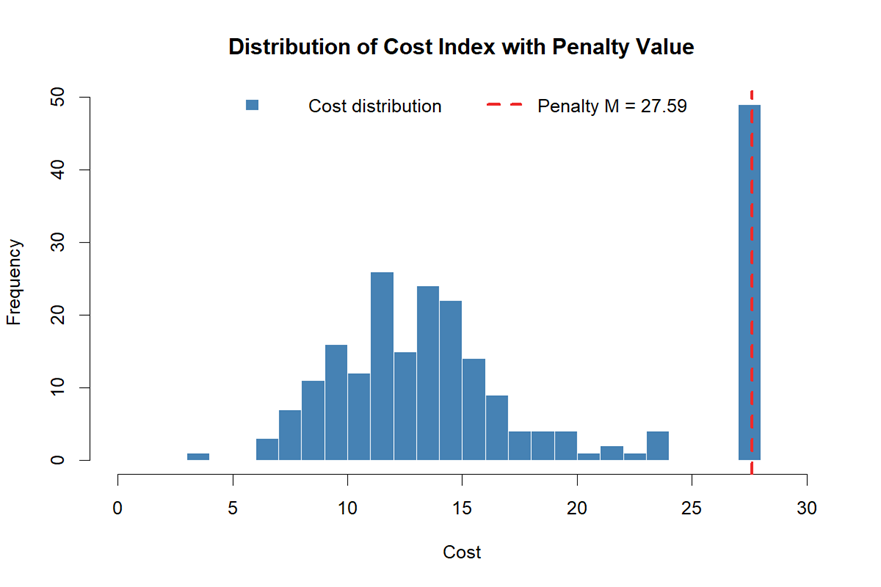
\includegraphics[width=0.85\textwidth]{figures/cost_index_penalty_distribution.png}
    \caption{Distribution of the generalised accessibility cost before normalisation, including penalty value}
    \label{fig:cost_index_penalty_distribution}
\end{figure}

Figure~\ref{fig:cost_index_penalty_distribution} shows the distribution of the pre-normalised generalised accessibility cost, with the assigned penalty value shown at \(M = 27.59\). The penalty value is positioned above the main distribution of route-feasible LSOA-campus pairs, ensuring that pairs with no feasible public transport route returned by the routing model are retained as the highest cost observations before min-max normalisation.

Finally, the weighted index was normalised using min-max scaling:

\[
I_l^{\text{norm}}
=
\frac{
I_l
-
\min\left(I_l\right)
}{
\max\left(I_l\right)
-
\min\left(I_l\right)
}.
\]

This yields values bounded in \([0,1]\), preserves relative differences in accessibility, and facilitates comparison across LSOAs. However, because min-max normalisation is calculated from the observed sample, the absolute value of \(I_l^{\text{norm}}\) is sample-dependent and would change if additional LSOAs or alternative destination assumptions were introduced.





\section{Results}

This chapter presents empirical findings addressing four research questions: the variation of deprivation among staff home locations; the relationship between deprivation and commuting behaviour; the spatial and campus-based variation of public transport accessibility; and the association between the generalised accessibility cost index, deprivation, and driving behaviour. These findings are interpreted in relation to transport disadvantage and accessibility, where mobility outcomes are shaped by the interaction between social inequality, residential location and transport provision (\hcite{lucas2012}{Lucas, 2012}), and to Welsh Government policy objectives around equitable access to sustainable transport (\hcite{welshgov2021active}{Welsh Government, 2021}).


\subsection{Staff distribution across deprivation}

Following GIS-based spatial filtering to the Cardiff local authority boundary, 840 staff were retained across 191 of Cardiff's 229 LSOAs, forming the final analytical sample.

\begin{figure}[H]
    \centering
    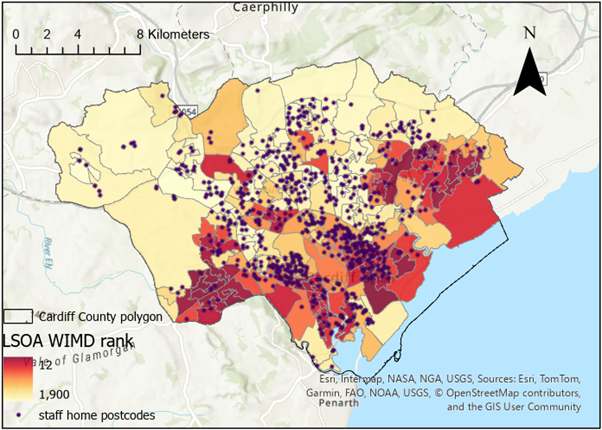
\includegraphics[width=0.85\textwidth]{figures/staff_distribution_wimd_map.png}
    \caption{Residential distribution of staff by LSOA WIMD rank}
    \label{fig:staff_distribution_wimd}
\end{figure}

The spatial distribution is non-uniform. While clustering is visible in central areas, there is a clear concentration in less deprived northern and western LSOAs. Conversely, fewer staff reside in the most deprived areas of south and east Cardiff, consistent with the occupational structure of a higher education workforce and with wider evidence linking socioeconomic position, residential location and transport opportunity (\hcite{lucas2012}{Lucas, 2012}).

\begin{figure}[H]
    \centering
    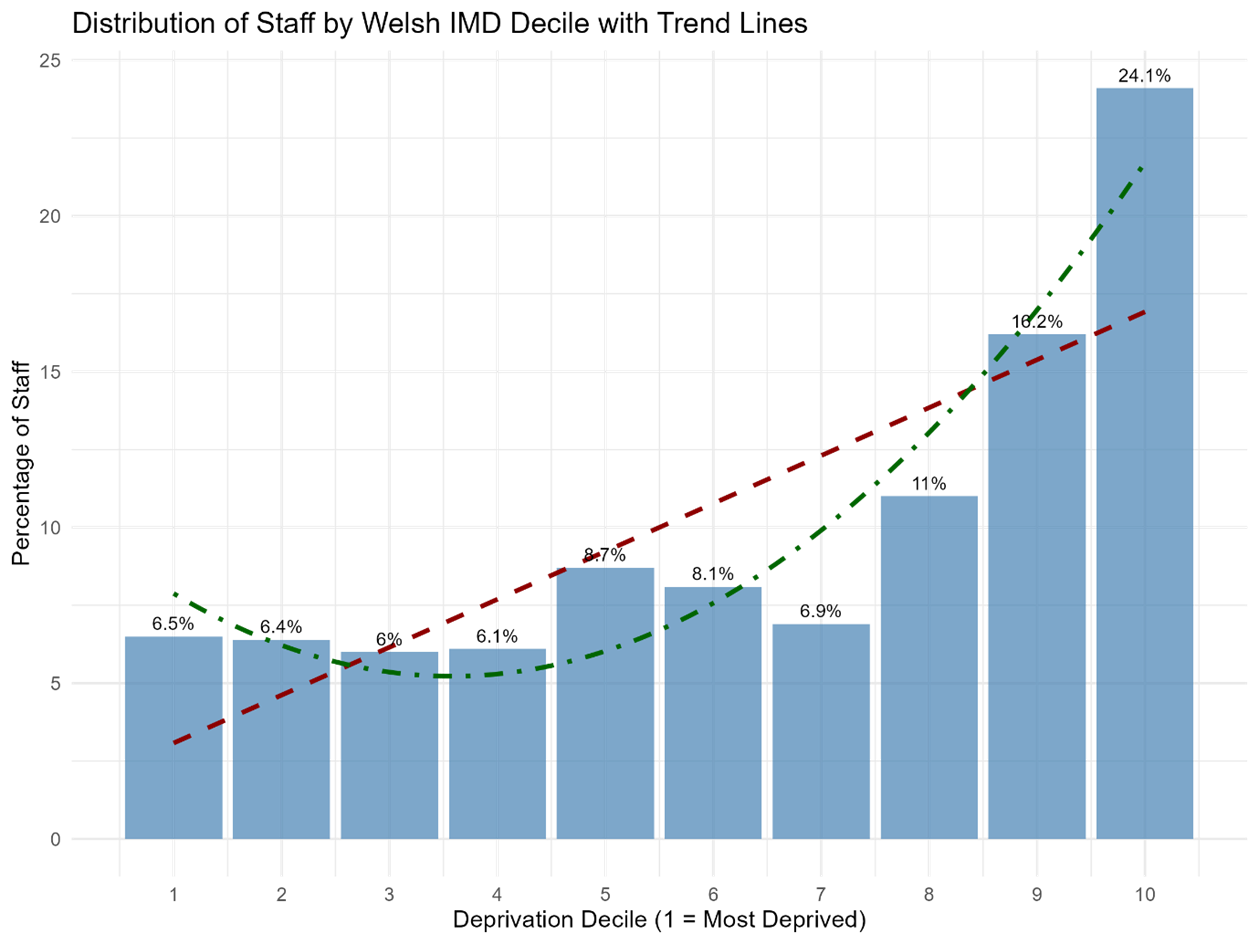
\includegraphics[width=0.85\textwidth]{figures/wimd_decile_distribution.png}
    \caption{Distribution of staff by WIMD decile}
    \label{fig:wimd_decile_distribution}
\end{figure}

The sample is skewed towards less deprived areas, with 24\% of Cardiff-based staff residing in decile 10 alone. The mean WIMD decile is 6.77, above the midpoint of 5.5, with positive skewness of 1.38. To characterise this gradient, linear and quadratic models of decile proportions were compared. The quadratic specification provides a better fit ($R^2 = 0.90$) than the linear model ($R^2 = 0.63$), identifying an inflection point around deciles 3-4. This supports a non-linear interpretation of staff residential distribution, with under-representation in more deprived neighbourhoods and concentration in less deprived areas.

\subsection{Deprivation and commuting behaviour}

\begin{figure}[H]
    \centering
    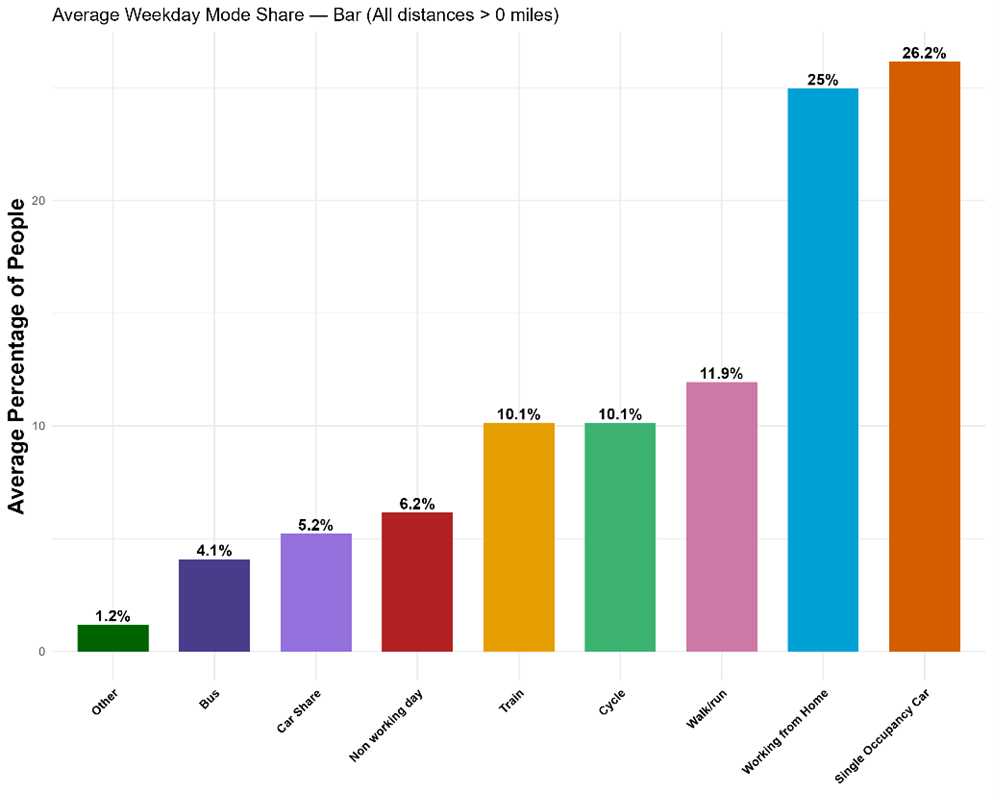
\includegraphics[width=0.7\textwidth]{figures/modal_split.png}
    \caption{Average weekday modal split of staff commuting}
    \label{fig:modal_split}
\end{figure}

Single-occupancy car (SOC) travel is the most frequent mode, accounting for 26.2\% of average weekday observations. This is followed by walking/running (11.9\%), cycling (10.1\%), train (10.1\%), car sharing (5.2\%), and bus (4.1\%). A combined 31.2\% of observations involve no commuting activity, consisting of working from home (25.0\%) and non-working days (6.2\%). As these non-commuting observations mechanically suppress unadjusted driving frequency, a WFH-adjusted measure is used in the subsequent analysis.

\begin{figure}[H]
    \centering
    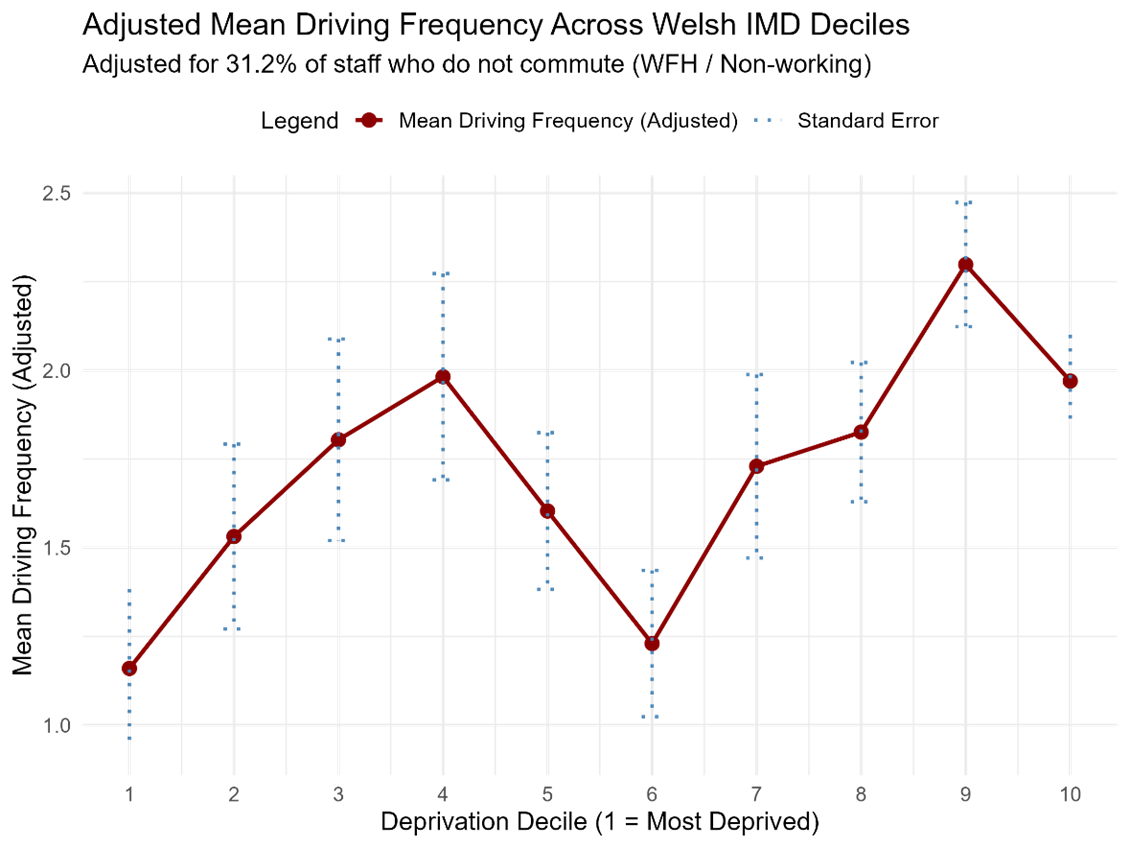
\includegraphics[width=0.7\textwidth]{figures/adjusted_driving_frequency_wimd.png}
    \caption{Adjusted mean SOC driving frequency by WIMD decile}
    \label{fig:adjusted_driving_wimd}
\end{figure}

Adjusting for non-commuting days increases mean driving frequency from 1.244 to 1.809 days per week but does not alter the overall deprivation pattern. A Welch's ANOVA, performed following a Fligner-Killeen test indicating unequal variance ($p < 0.001$), shows a significant difference in driving frequency across deprivation deciles ($F = 3.05$, $p = 0.0015$). The non-monotonic relationship suggests that commuting behaviour is governed by the interaction of residential location, car availability and public transport accessibility rather than a purely linear deprivation gradient.

\subsection{Bus accessibility and deprivation}

\begin{figure}[H]
    \centering
    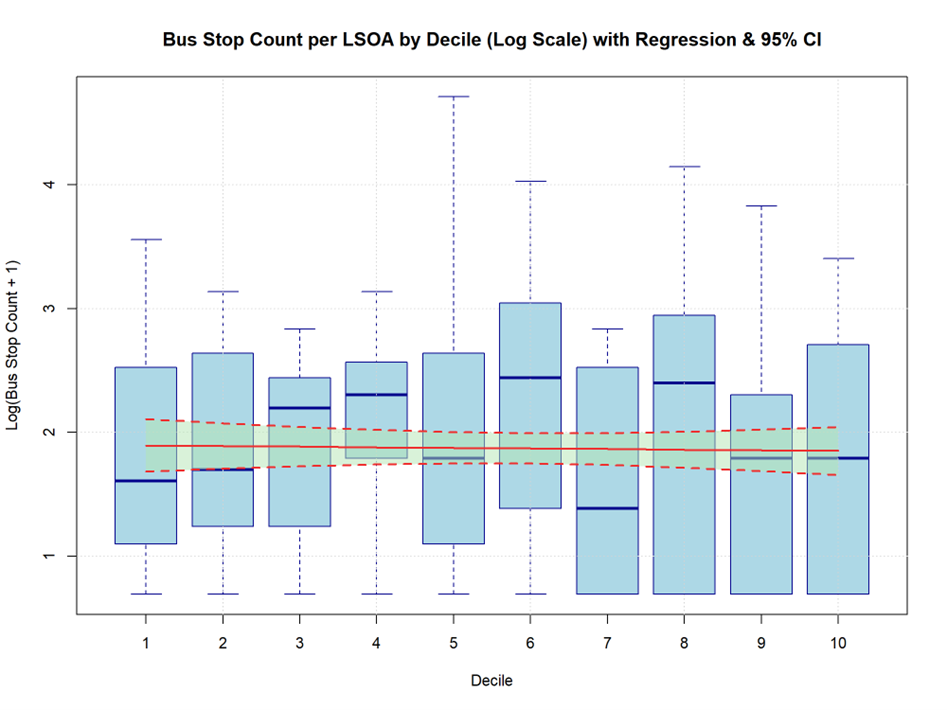
\includegraphics[width=0.78\textwidth]{figures/bus_stop_counts_wimd.png}
    \caption{Service-weighted bus stop counts per LSOA by WIMD decile}
    \label{fig:bus_stop_counts_wimd}
\end{figure}

A total of 2,028 GTFS service records were identified, covering 180 of Cardiff's 229 LSOAs. These should be interpreted as service-weighted records rather than unique physical stop locations, as GTFS data include multiple records by route, direction and stop pattern. Log transformation was applied to compress the variance of this right-skewed distribution. The fitted relationship is effectively flat, with a wide 95\% confidence interval and a Spearman correlation of $-0.018$. Within-decile variation substantially exceeds between-decile variation, confirming that service intensity is driven more by local network topology than deprivation. This supports the argument that stop-based measures are inadequate as standalone accessibility indicators, justifying the transition to a route-based generalised cost index (\hcite{handy1997}{Handy and Niemeier, 1997}).
\newpage

\subsection{Travel time baseline and spatial accessibility}

Public transport travel times were modelled across eight weekday departure hours between 07:00 and 19:00. Figures~\ref{fig:time_budget_maps} show public transport time-budget maps for Heath Park and Cathays, based on Cardiff bus stop points with a 400 m buffer representing an acceptable walking distance to a bus stop. Because both maps use the same bus stop catchments, the spatial coverage is identical; the difference lies in the travel-time classification assigned to each catchment.

\begin{figure}[H]
    \centering

    \begin{subfigure}[t]{0.495\textwidth}
        \centering
        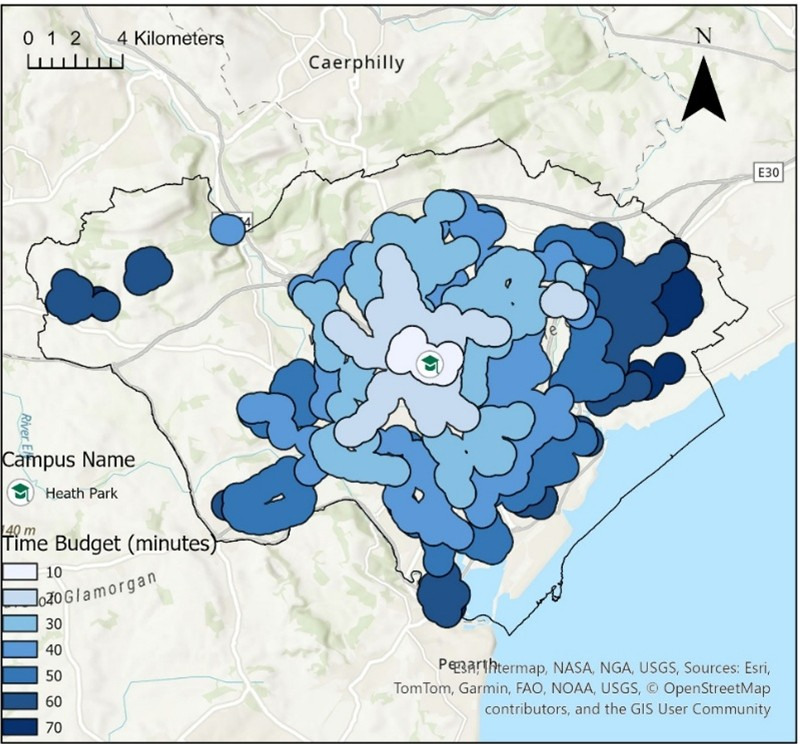
\includegraphics[width=\linewidth]{figures/heath_time_budget_map.jpg}
        \caption{Heath Park Campus}
        \label{fig:heath_time_budget}
    \end{subfigure}
    \begin{subfigure}[t]{0.495\textwidth}
        \centering
        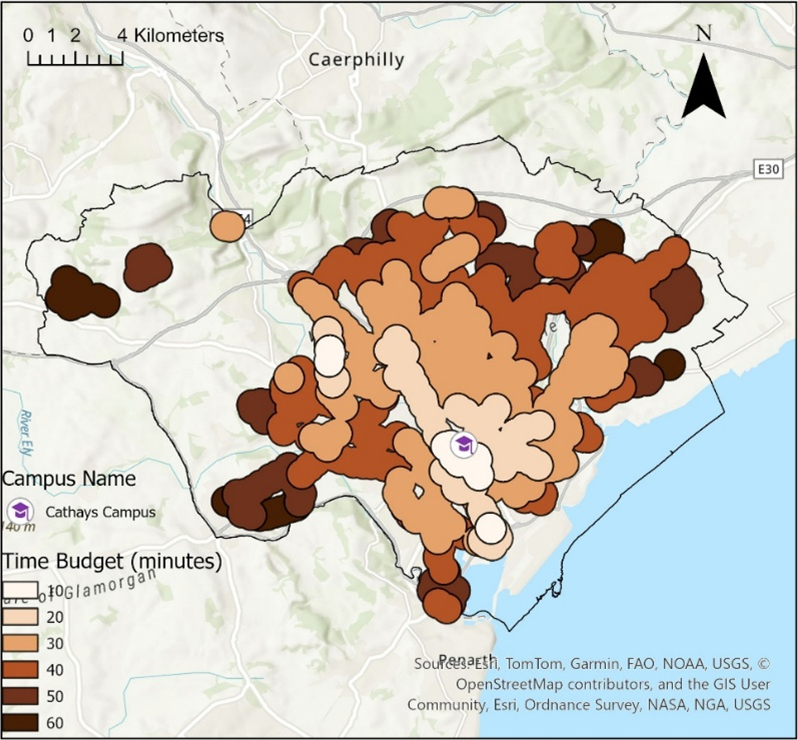
\includegraphics[width=\linewidth]{figures/cathays_time_budget_map.png}
        \caption{Cathays Campus}
        \label{fig:cathays_time_budget}
    \end{subfigure}

    \caption{Public transport time-budget maps to Heath Park and Cathays campuses using 400 m bus stop catchments}
    \label{fig:time_budget_maps}
\end{figure}

Public transport time-budget maps were constructed using 400 m bus stop catchments, the standard distance used in transport planning to approximate walking access to bus services (\hcite{foda2010}{Foda and Osman, 2010}). This catchment was used only for the map-based accessibility surfaces; the accessibility cost index itself was calculated at LSOA level so that all areas of Cardiff could be compared on a consistent spatial unit.

Cathays has a larger concentration of low travel-time buffers around the city centre, reflecting its position within the dense inner-city bus network. Heath Park exhibits a less favourable travel-time profile across the same bus stop catchment network, with more locations falling into higher time-budget bands. Much of south, west and outer Cardiff requires substantially longer journeys to Heath, with several areas falling into the 50-70 minute bands. This structural asymmetry supports the decision to calculate campus-specific costs before combining them into a staff-weighted accessibility index.

\begin{figure}[H]
    \centering
    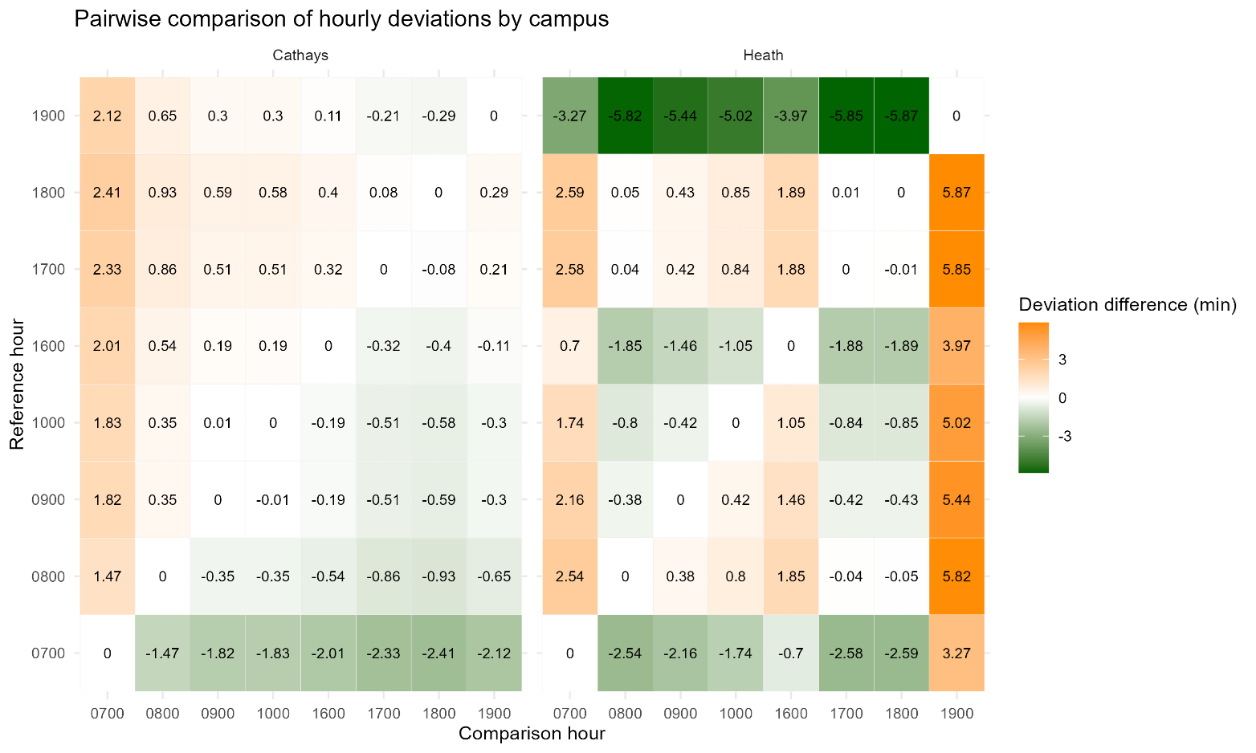
\includegraphics[width=0.78\textwidth]{figures/temporal_stability_travel_time.png}
    \caption{Temporal stability of public transport travel time by campus}
    \label{fig:temporal_stability}
\end{figure}

Deviations across departure periods are approximately $\pm 2$ minutes for Cathays and $\pm 3$ minutes for Heath. Additional campus-level summary statistics for the top-three route measure are reported in Appendix~\ref{app:graphs_stats}, Table~\ref{tab:top3_time_sd_summary}. This consistency supports the temporal averaging approach used in index construction.

\begin{figure}[H]
    \centering
    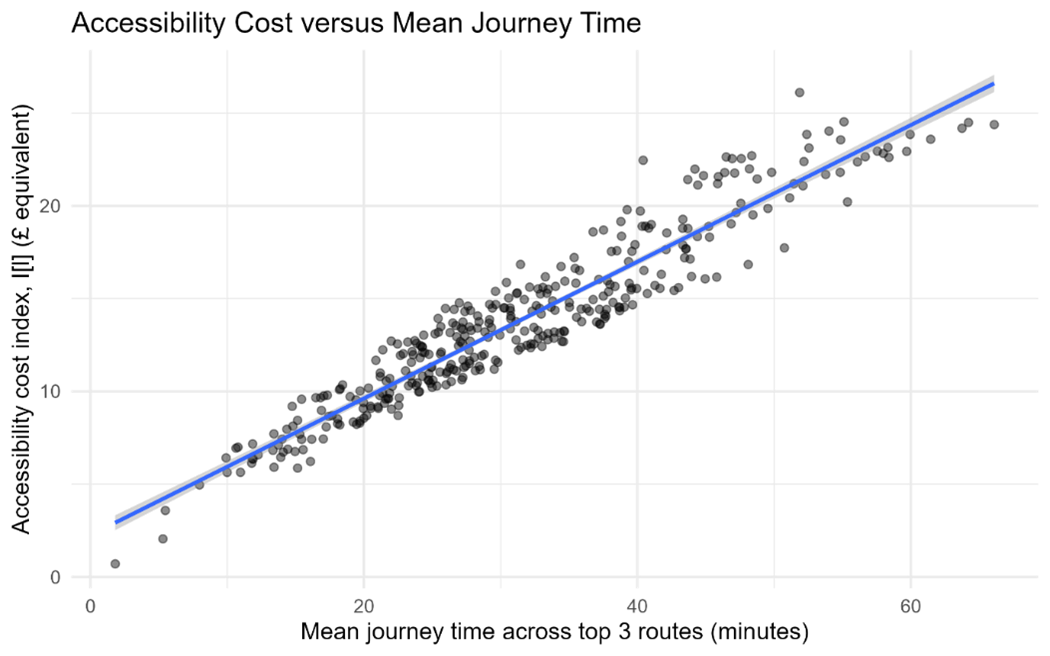
\includegraphics[width=0.78\textwidth]{figures/journey_time_index_relationship.png}
    \caption{Relationship between journey time and generalised accessibility cost index}
    \label{fig:journey_time_index}
\end{figure}

There is a strong, statistically significant positive relationship between mean journey time and the generalised accessibility cost index ($r = 0.949$, $\rho = 0.946$, $p < 2.2 \times 10^{-16}$). Journey time was monetised using the Department for Transport's commuting value of time of \pounds16 per hour, equivalent to approximately \pounds0.267 per minute (\hcite{hmtreasury2025}{HM Treasury, 2025}). Residual variation around the fitted line reflects walking time, waiting and interchange burden, temporal variability and fares. The index therefore functions as a monetised transformation of time burden, adjusted for route quality and monetary cost, consistent with generalised cost approaches used in transport appraisal guidance.

\begin{figure}[H]
    \centering
    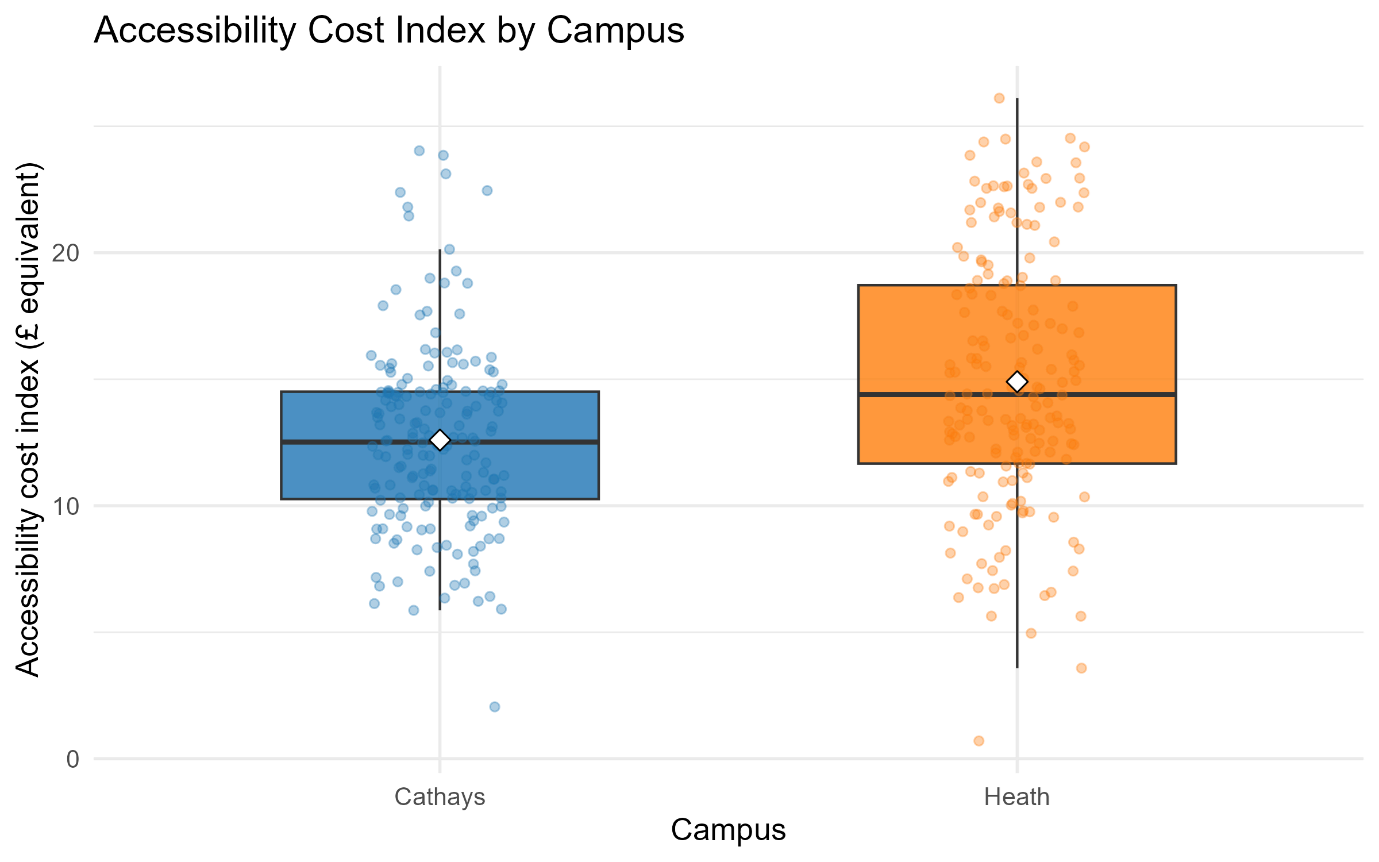
\includegraphics[width=0.78\textwidth]{figures/accessibility_cost_by_campus.png}
    \caption{Accessibility cost index by campus}
    \label{fig:accessibility_cost_campus}
\end{figure}

Accessibility costs differ systematically between campuses. Heath exhibits higher mean costs (\pounds14.90) than Cathays (\pounds12.59), and the wider interquartile range at Heath indicates greater variability in accessibility conditions. A Welch two-sample t-test confirms that this difference is statistically significant ($t = -4.95$, $p < 0.001$), supporting the inclusion of campus weighting as a factoring variable in the generalised accessibility cost index.

\subsection{Accessibility cost and driving behaviour}

\subsubsection{Descriptive distributions and index output}

The normalised accessibility cost index is right-skewed across the 840 staff residential locations (Figure~\ref{fig:index_distribution}). Most observations fall between 0.15 and 0.55, while the spike at 1.0 represents LSOAs assigned the inaccessibility penalty where no feasible public transport route was identified. The mean value of the index (0.458) therefore exceeds the median (0.382). These observations are retained because excluding them would remove the least accessible areas from the analysis and understate the relationship between poor accessibility and commuting behaviour.

\begin{figure}[H]
    \centering
    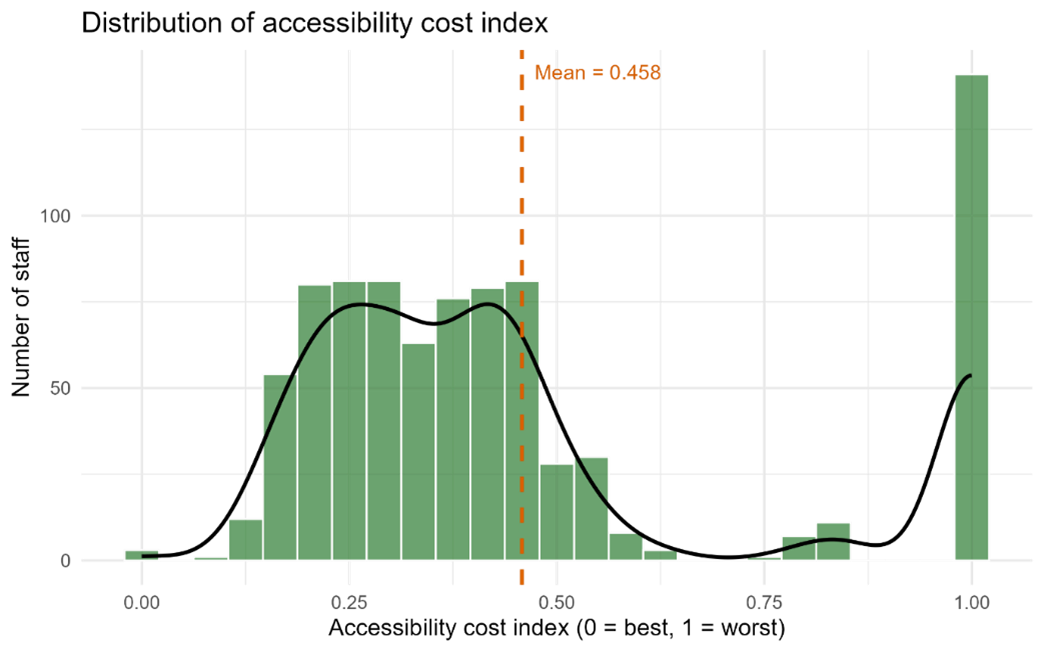
\includegraphics[width=0.78\textwidth]{figures/index_distribution.png}
    \caption{Distribution of normalised accessibility cost index across staff residential locations ($n = 840$), with mean = 0.458}
    \label{fig:index_distribution}
\end{figure}

The spatial pattern underlying this distribution is shown in Figure~\ref{fig:index_spatial_distribution}. Accessibility costs are lowest in LSOAs surrounding Cathays and Heath and along the main bus corridors extending north and east from the city centre. Lower-cost areas cluster around Cathays, Roath, Heath and Gabalfa, reflecting the dense bus network serving these inner-city areas and reducing both walking and in-vehicle journey times.

Costs increase with distance from the urban core, but the gradient is asymmetric. Western Cardiff, including Canton, Fairwater, Llandaff North and areas beyond the River Ely, forms the largest high-cost cluster. Despite being relatively close to the campuses in straight-line terms, these areas face higher generalised costs because routes are less direct, often require interchange, or involve longer walking and waiting components. Southern and coastal areas also show elevated costs, particularly around Cardiff Bay, where routes to Heath Park are more indirect.

This directly addresses Research Question 2, demonstrating that public transport accessibility is not simply a function of distance from campus, but is shaped by Cardiff’s radial bus network. The darkest peripheral LSOAs correspond to penalty-assigned areas with no feasible route, indicating locations with insufficient public transport coverage within the routing assumptions.

\begin{figure}[H]
    \centering
    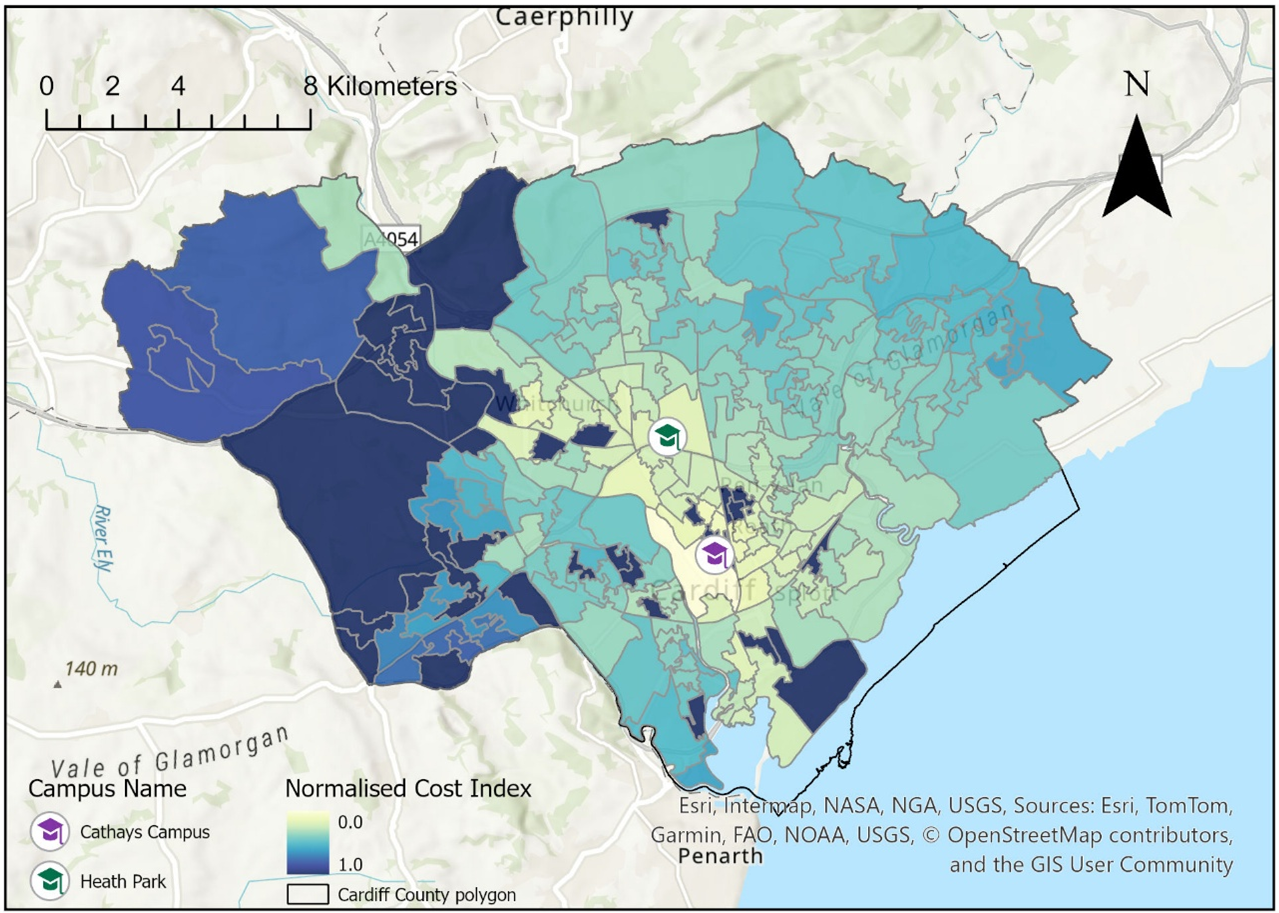
\includegraphics[width=0.85\textwidth]{figures/index_spatial_distribution.png}
    \caption{Spatial distribution of the normalised accessibility cost index across Cardiff LSOAs, with campus locations. Yellow indicates low cost and best accessibility; dark blue indicates high cost or penalty-assigned areas and worst accessibility}
    \label{fig:index_spatial_distribution}
\end{figure}

Crucially, the high-cost western LSOAs are not the most deprived areas of Cardiff. Deprivation in Cardiff is concentrated more strongly in the south and inner east, which explains why the correlation between the cost index and WIMD rank is moderate rather than strong. Accessibility disadvantage and socioeconomic deprivation are therefore related but spatially distinct in this context, motivating the controlled regression analysis below and underpinning the interaction results in Section~\ref{sec:interaction_accessibility_deprivation}.

\begin{figure}[H]
    \centering
    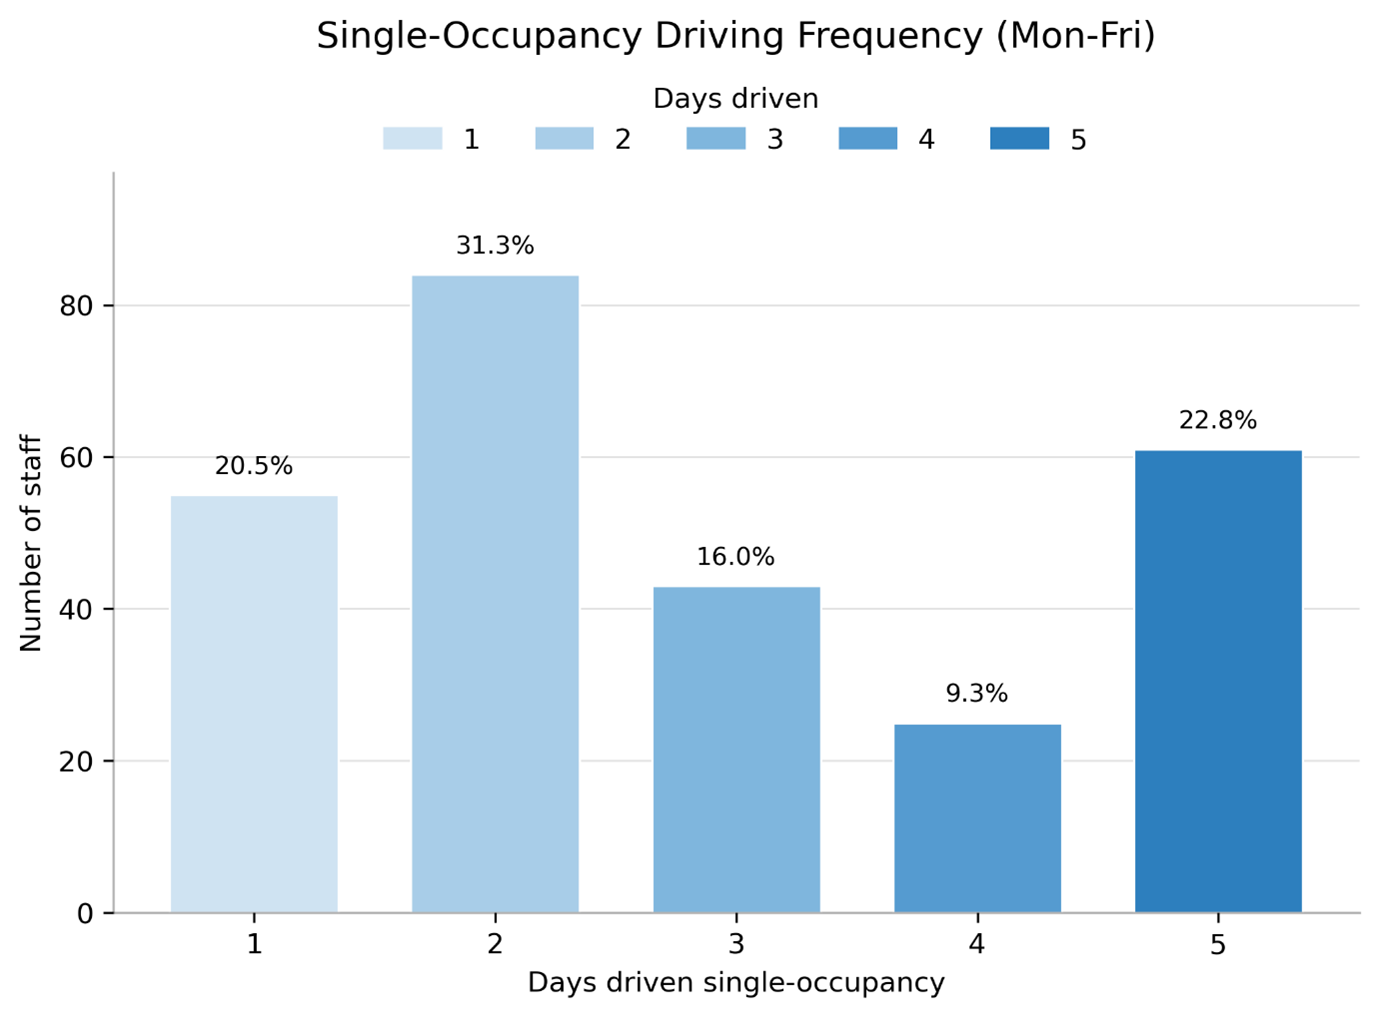
\includegraphics[width=0.7\textwidth]{figures/soc_driving_frequency.png}
    \caption{Distribution of single-occupancy driving frequency among Cardiff SOC-driving staff}
    \label{fig:soc_driving_frequency}
\end{figure}

Figure~\ref{fig:soc_driving_frequency} shows that among Cardiff staff who drive single-occupancy, the most common frequency is two days per week (31.3\%), although 22.8\% drive alone every weekday, indicating a smaller but clearly car-dependent group.

\begin{figure}[H]
    \centering
    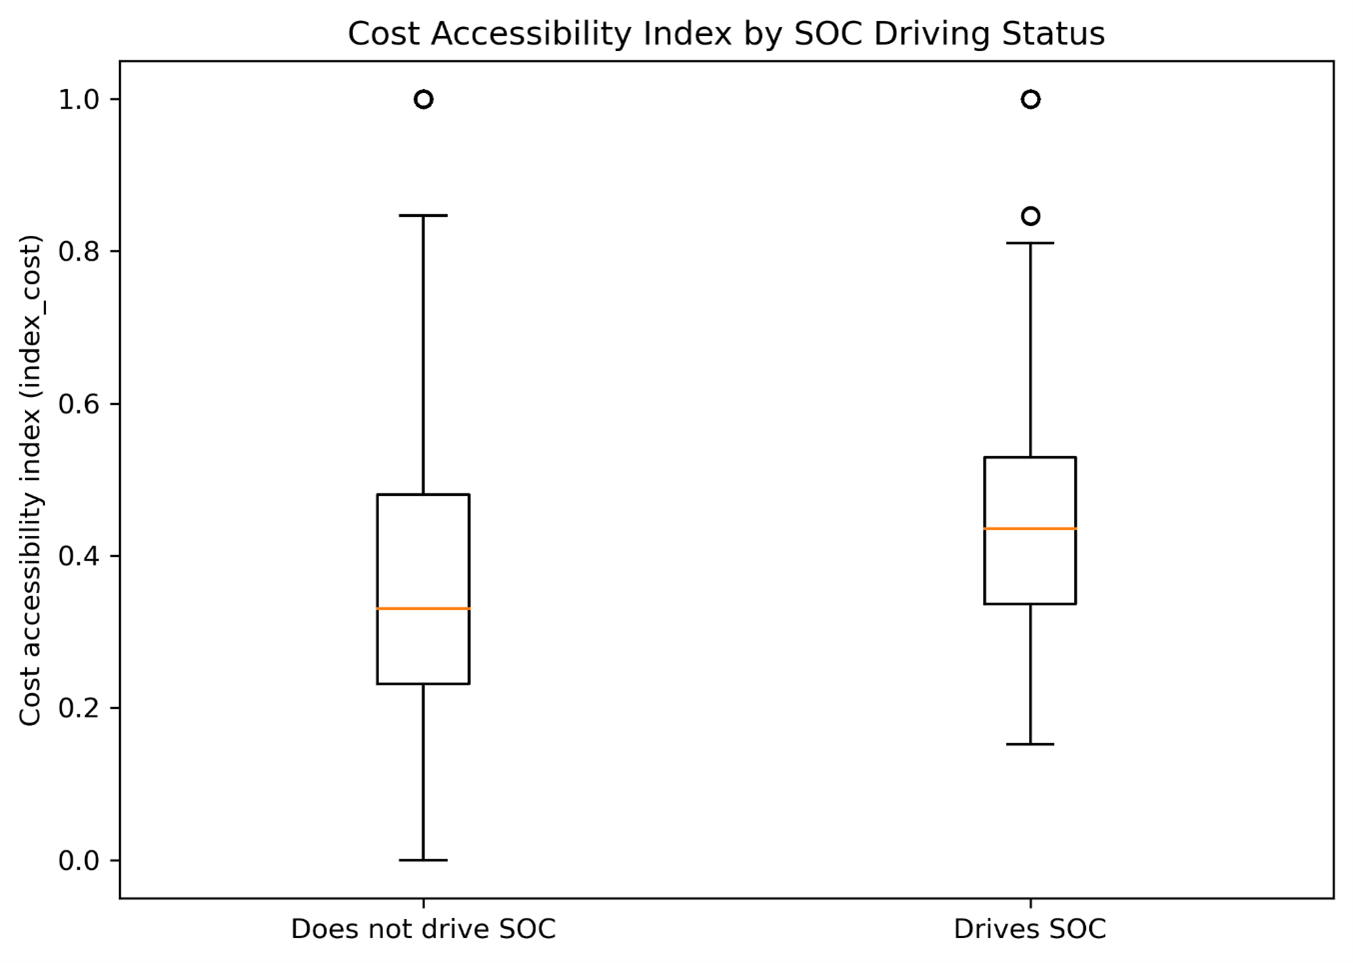
\includegraphics[width=0.6\textwidth]{figures/index_by_soc_driving_status.png}
    \caption{Cost accessibility index by single-occupancy car driving status among Cardiff staff ($n = 840$)}
    \label{fig:index_by_soc_status}
\end{figure}

Figure~\ref{fig:index_by_soc_status} compares the distribution of the normalised accessibility cost index between staff who report single-occupancy car driving and those who do not. SOC drivers have a higher median index score (0.435) than non-SOC drivers (0.331), indicating poorer public transport accessibility among car users. A Mann-Whitney U test confirms that this difference is statistically significant ($U = 56{,}628.5$, $p < 0.001$), with a rank-biserial correlation of 0.261, indicating a small-to-moderate effect size. However, the distributions overlap substantially, showing that accessibility cost is a contributory rather than deterministic factor in mode choice.


\subsubsection{Bivariate relationships}

\begin{figure}[H]
    \centering
    \begin{subfigure}{0.48\textwidth}
        \centering
        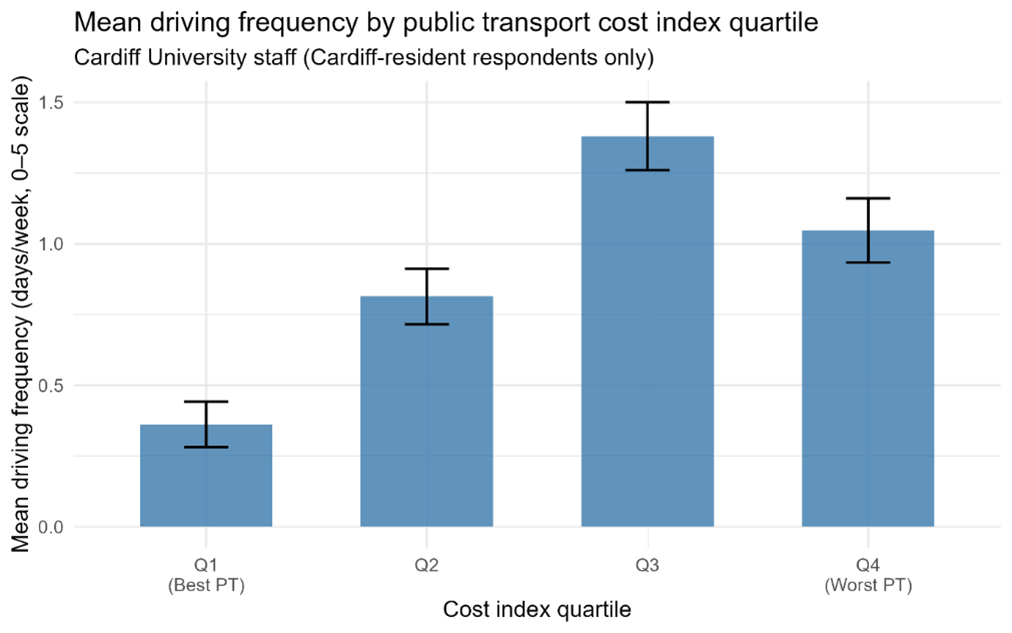
\includegraphics[width=\textwidth]{figures/driving_by_cost_quartile.png}
        \caption{Mean driving frequency by accessibility cost quartile, with standard error bars}
        \label{fig:driving_by_cost_quartile}
    \end{subfigure}
    \hfill
    \begin{subfigure}{0.48\textwidth}
        \centering
        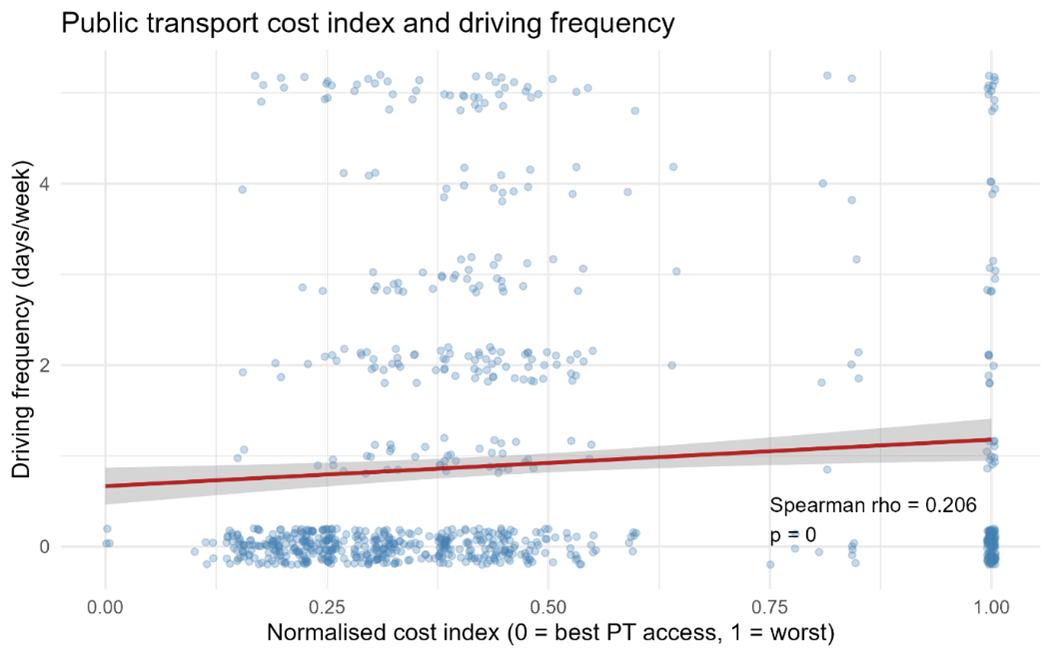
\includegraphics[width=\textwidth]{figures/index_driving_scatter.png}
        \caption{Driving frequency and accessibility cost index, with fitted line}
        \label{fig:index_driving_scatter}
    \end{subfigure}
    \caption{Bivariate relationship between accessibility cost and single-occupancy driving frequency}
    \label{fig:bivariate_cost_driving}
\end{figure}

Figure~\ref{fig:bivariate_cost_driving} shows a statistically significant positive association between accessibility cost and driving frequency (Spearman's $\rho = 0.206$, $p < 0.001$). Mean driving frequency increases from 0.36 days per week in the lowest-cost quartile to 1.38 in the third quartile, representing a substantial increase in car use as accessibility worsens. The decline to 1.05 in the fourth quartile suggests non-monotonic behaviour, potentially reflecting structural adaptation, such as relocation, hybrid working, or reduced commuting among staff facing extreme levels of inaccessibility.




\subsubsection{Regression analysis}

\begin{table}[H]
\centering
\caption{OLS regression models predicting driving frequency among Cardiff-based staff}
\label{tab:ols_driving_models}
\begin{tabular}{lccc}
\hline
 & M1 & M2 & M3 \\
 & Cost index only & Cost index + WIMD rank & Fare + WIMD rank \\
\hline
Intercept & 0.666*** & 0.331* & 0.450** \\
          & (0.104)  & (0.136) & (0.140) \\
Accessibility cost index & 0.513** & 0.370. & -- \\
                         & (0.194) & (0.197) & -- \\
WIMD rank & -- & 0.000342*** & 0.000372*** \\
          & -- & (0.000091) & (0.000091) \\
Fare index & -- & -- & 0.030 \\
           & -- & -- & (0.201) \\
\hline
Observations & 840 & 840 & 840 \\
Residual SE & 1.546 & 1.535 & 1.538 \\
Adjusted $R^2$ & 0.007 & 0.022 & 0.018 \\
AIC & 3120 & 3108 & 3112 \\
F-statistic & 6.965** & 10.590*** & 8.793*** \\
\hline
\multicolumn{4}{l}{\footnotesize Standard errors in parentheses.} \\
\multicolumn{4}{l}{\footnotesize Significance: *** $p<0.001$, ** $p<0.01$, * $p<0.05$, . $p<0.10$.} \\
\end{tabular}
\end{table}

In the baseline model (M1), the accessibility cost index is a positive and statistically significant predictor of driving frequency (\(\beta = 0.513\), \(p < 0.01\)). As the index is normalised between 0 and 1, this coefficient suggests that moving from the lowest to the highest observed accessibility cost is associated with approximately 0.51 additional single-occupancy driving days per week, on average. However, explanatory power is limited (adjusted \(R^2 = 0.007\)), indicating that accessibility alone explains only a small proportion of variation in commuting behaviour.

In M2, WIMD rank is introduced to control for deprivation. WIMD rank is statistically significant (\(p < 0.001\)), while the accessibility cost index remains positive but weakens to marginal significance (\(p = 0.060\)). This suggests that part of the observed relationship between accessibility and driving reflects underlying socioeconomic and spatial patterns. Although M2 has the lowest AIC of the three models, its explanatory power remains limited (adjusted \(R^2 = 0.022\)).

In M3, fare is included alongside WIMD rank as an alternative to the composite accessibility index. Fare is not statistically significant (\(p = 0.883\)), while WIMD rank remains statistically significant. Model fit is weaker than in M2, indicating that fare alone is not an adequate substitute for the composite accessibility index.

Overall, accessibility cost is a statistically significant but modest predictor of driving behaviour. Higher costs are associated with increased single-occupancy car use, but most variation remains unexplained by these models. This likely reflects omitted individual-level factors such as car ownership, parking access, job role, household constraints and work flexibility. WIMD rank plays a more substantial role than accessibility in this sample, although the overall explanatory power of all three models remains low.


\subsection{Comparative performance of accessibility measures}

\begin{table}[H]
\centering
\caption{Spearman correlations between accessibility measures and driving frequency among Cardiff staff ($n = 840$)}
\label{tab:accessibility_measure_correlations}
\begin{tabular}{lcc}
\hline
Variable & Spearman's $\rho$ & Interpretation \\
\hline
Accessibility cost index & 0.206*** & Strongest association \\
Fare (normalised)        & 0.111**  & Weak association \\
Bus stop count           & 0.076*   & Very weak association \\
Bus departures           & -0.030   & No association \\
\hline
\multicolumn{3}{l}{\footnotesize Significance: *** $p<0.001$, ** $p<0.01$, * $p<0.05$.} \\
\end{tabular}
\end{table}

To assess whether simpler measures of transport provision capture commuting behaviour, the accessibility cost index was compared with fare, bus stop density and total service departures.

The cost index shows the strongest association with driving frequency (Spearman's $\rho = 0.206$), followed by fare ($\rho = 0.111$). While fare shows a weak positive correlation with driving frequency, it is not statistically significant when controlling for deprivation. This suggests that the observed relationship between fare and driving reflects underlying socioeconomic patterns rather than an independent effect of fare on behaviour. In contrast, stop density exhibits only a very weak positive relationship ($\rho = 0.076$), while total departures show no meaningful relationship ($\rho = -0.030$).

These results indicate that service-based measures of transport provision do not adequately capture accessibility. While stop density and service frequency describe infrastructure availability, they do not reflect the ease of completing a journey. However, the association remains modest, so the index should be interpreted as a stronger comparative accessibility measure rather than a complete predictor of commuting behaviour.

\subsection{Interaction between accessibility and deprivation}
\label{sec:interaction_accessibility_deprivation}

\begin{figure}[H]
    \centering
    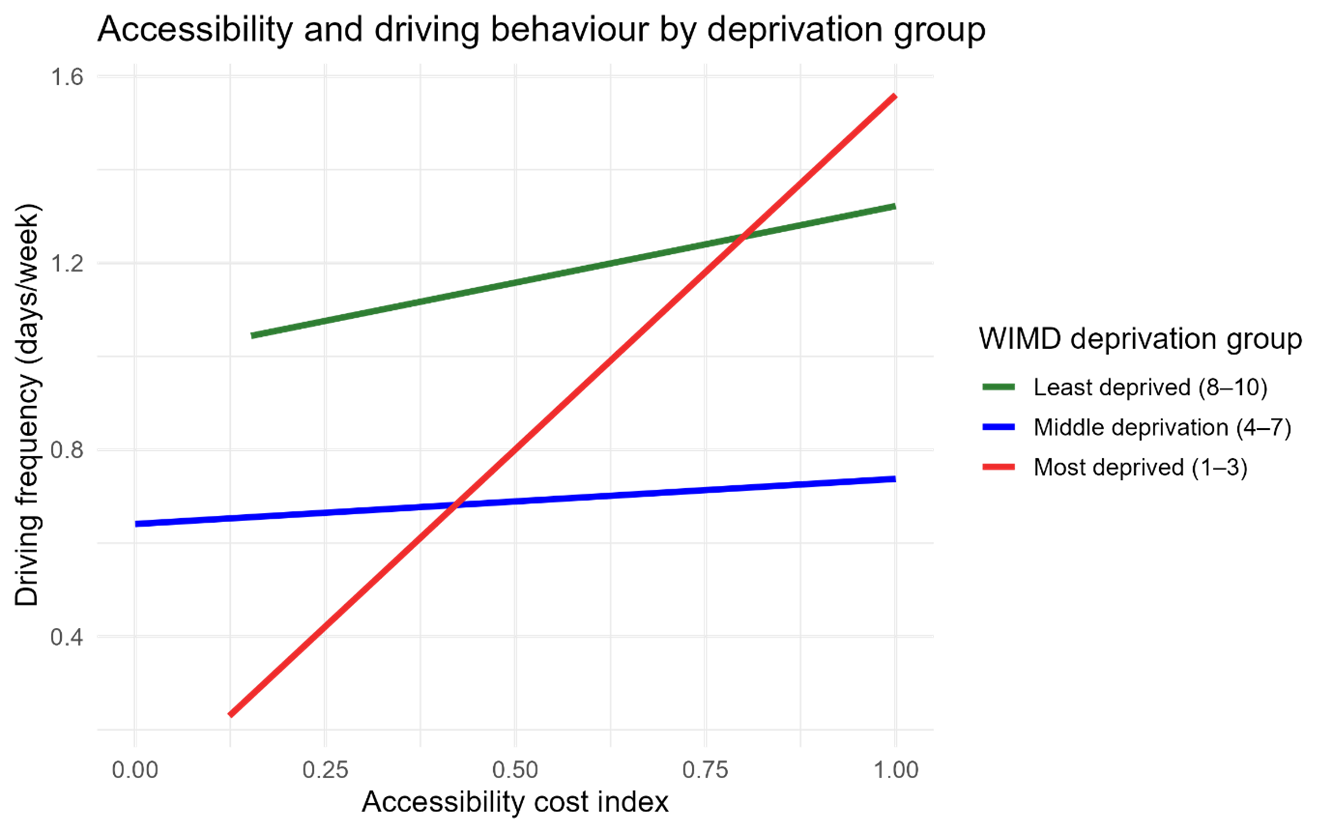
\includegraphics[width=0.76\textwidth]{figures/accessibility_deprivation_interaction.png}
    \caption{Predicted driving frequency by accessibility cost index and deprivation group}
    \label{fig:accessibility_deprivation_interaction}
\end{figure}

To assess whether the relationship between accessibility cost and driving behaviour varies across the socioeconomic distribution, an interaction model was estimated between the cost index and WIMD decile. Staff were grouped into three bands: most deprived (deciles 1-3), middle (4-7), and least deprived (8-10).

The accessibility cost index remains a statistically significant predictor of driving frequency ($\beta = 1.31$, $p = 0.012$), and deprivation is also significant ($\beta = 0.126$, $p < 0.001$), with less deprived staff exhibiting higher baseline driving. The interaction term is negative and marginally significant ($\beta = -0.136$, $p = 0.051$), indicating that the effect of accessibility cost weakens as deprivation decreases.

Figure~\ref{fig:accessibility_deprivation_interaction} illustrates this relationship. Staff in the most deprived group exhibit the lowest baseline driving but the steepest gradient, with driving frequency increasing sharply as accessibility cost rises. In contrast, the least deprived group displays higher baseline driving across all cost levels but a flatter gradient, suggesting that their behaviour is less sensitive to changes in accessibility.

This pattern indicates that accessibility cost is a more important determinant of commuting behaviour in more deprived groups, where public transport is more likely to represent a constrained choice rather than a preference. The marginal significance of the interaction term should be interpreted with caution; however, the direction and consistency of the pattern provide suggestive evidence of heterogeneous behavioural responses across the socioeconomic distribution.

\subsection{Robustness and sensitivity checks}

\begin{table}[H]
\centering
\caption{Sensitivity of accessibility cost values to value-of-time and waiting-time assumptions}
\label{tab:sensitivity_checks}
\begin{tabular}{cccccc}
\hline
Value of time (\pounds/hr) & Wait weight & Mean & Median & SD & Max \\
\hline
12 & 1.5 & 11.0 & 10.7 & 3.61 & 20.7 \\
12 & 2.0 & 11.2 & 10.8 & 3.84 & 21.6 \\
16 & 1.5 & 13.7 & 13.3 & 4.57 & 26.1 \\
16 & 2.0 & 14.1 & 13.5 & 4.86 & 27.3 \\
20 & 1.5 & 16.5 & 15.9 & 5.53 & 31.5 \\
20 & 2.0 & 16.9 & 16.2 & 5.89 & 32.9 \\
\hline
\end{tabular}
\end{table}

Sensitivity analysis was conducted by varying the value of time (\pounds12, \pounds16 and \pounds20 per hour) and the waiting-time weight (1.5 and 2.0). While absolute index values increase under higher parameter assumptions, the relative distribution of accessibility costs remains broadly stable. This indicates that the results are not sensitive to reasonable alternative specifications.

Temporal variation in journey times is limited, with differences across departure hours generally within approximately $\pm 2$-$3$ minutes. This supports the use of averaged travel times in the index. The penalty value assigned to LSOAs with no feasible public transport routes ensures that these areas are retained in the analysis. Although this affects the upper bound of the distribution, it does not materially alter the relative ordering of accessible areas. The value-of-time assumption is the dominant driver of variation in accessibility cost values. Increasing the value of time from \pounds12 to \pounds20 per hour raises the mean cost substantially, whereas increasing the waiting-time weight from 1.5 to 2.0 produces only a relatively small increase. This indicates that the index is more sensitive to the monetisation of travel time than to plausible changes in the residual waiting/interchange weighting.

Overall, the accessibility cost index shows limited sensitivity to parameter variation and modelling assumptions, supporting its use as a stable comparative measure of public transport accessibility.

\subsection{Policy implications: incentive preferences and accessibility context}

The preceding analysis establishes that accessibility cost is a statistically significant predictor of driving behaviour. Although these incentive responses are not used directly in the construction of the accessibility cost index, they provide useful contextual evidence on whether the barriers captured by the index, particularly fare burden and journey inconvenience, are reflected in staff preferences for sustainable travel interventions. This section examines whether staff incentive preferences are consistent with that finding, using survey responses on barriers to modal shift to assess the face validity of the accessibility cost framework and its policy implications.

\begin{figure}[H]
    \centering
    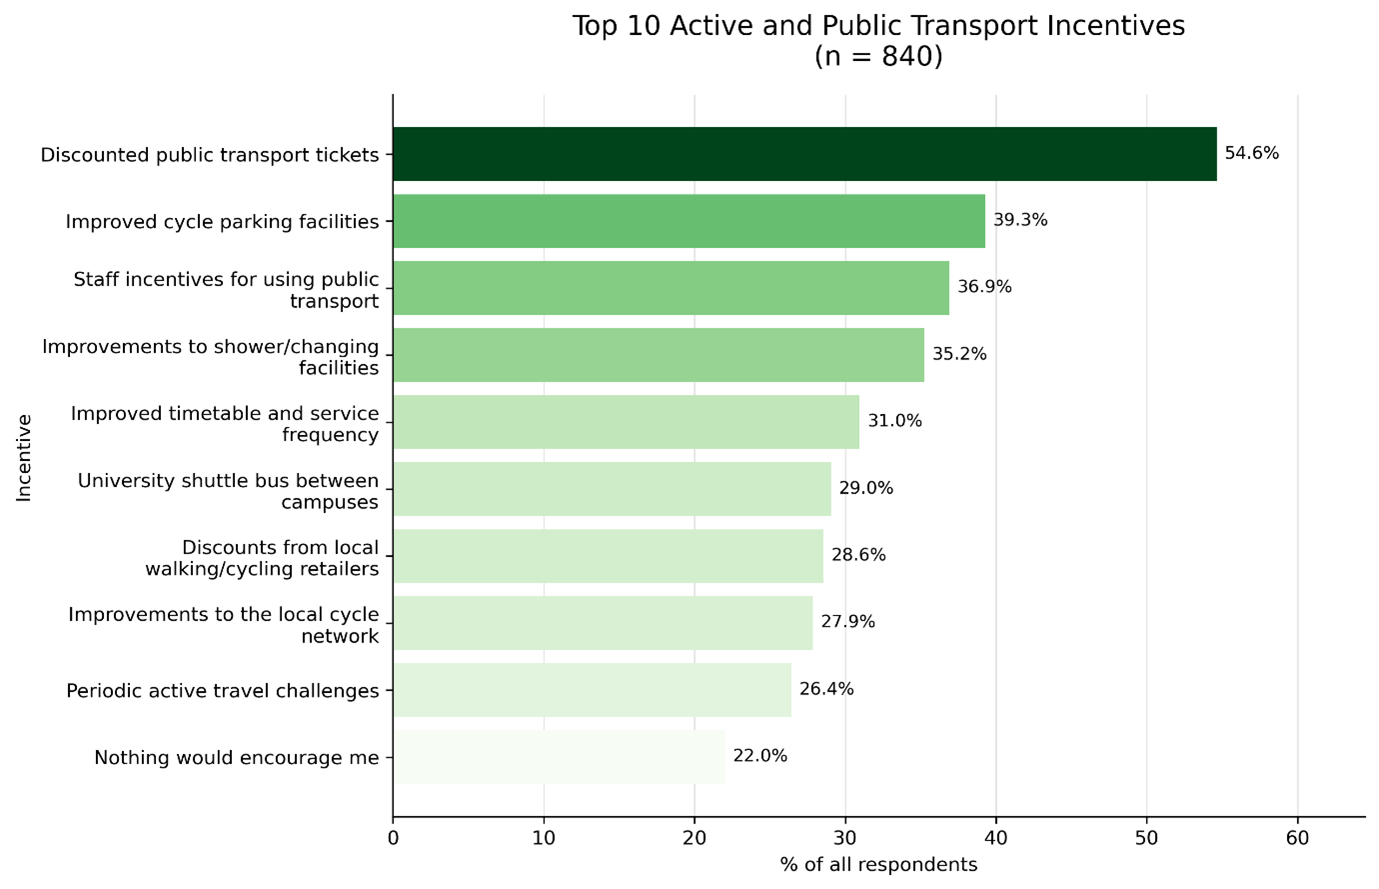
\includegraphics[width=0.86\textwidth]{figures/top10_incentives.png}
    \caption{Top 10 active travel and public transport incentives selected by Cardiff University staff ($n = 840$)}
    \label{fig:top10_incentives}
\end{figure}

Figure~\ref{fig:top10_incentives} presents the ten most frequently selected incentives among the matched sample. Discounted public transport tickets were the dominant preference, selected by 54.6\% of respondents, followed by improved cycle parking (39.3\%), staff incentives for using public transport (36.9\%) and shower/changing facilities (35.2\%). This is consistent with the earlier finding that transport cost and accessibility barriers are relevant to single-occupancy driving, although stated preferences should not be interpreted as direct evidence of behavioural change. The prominence of cycling and end-of-trip facilities shows that modal shift also depends on practical infrastructure improvements. The university shuttle bus between campuses (29.0\%) is also notable given the poorer accessibility observed for Heath Park, suggesting that campus-specific interventions may be needed alongside wider public transport improvements. A further 22.0\% selected ``nothing would encourage me'', indicating a limit to the level of modal shift achievable through incentives alone.

\begin{figure}[H]
    \centering
    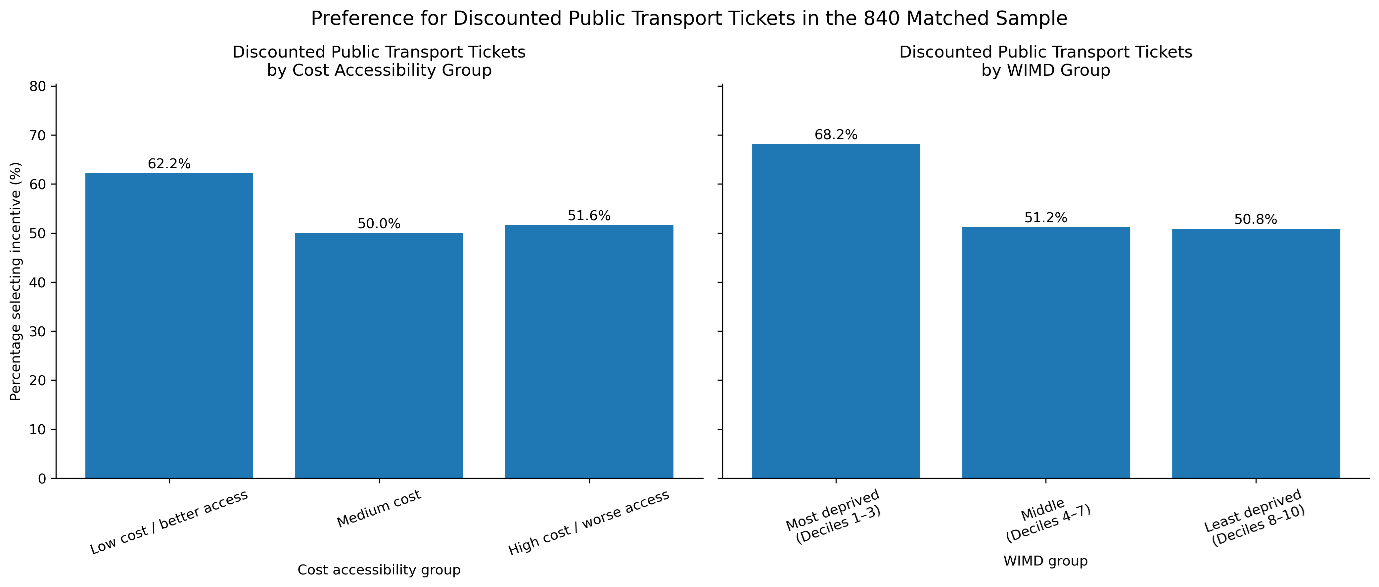
\includegraphics[width=0.90\textwidth]{figures/discounted_pt_by_cost_wimd.png}
    \caption{Support for discounted public transport tickets by accessibility cost and deprivation group}
    \label{fig:discounted_pt_cost_wimd}
\end{figure}

Discounted public transport tickets were the most commonly selected incentive. Support for this option varied significantly by accessibility cost group ($\chi^2(2) = 9.959$, $p = 0.0069$), and was highest among staff in the low-cost group. This suggests that fare discounts are most attractive where public transport is already relatively viable, rather than in the highest-cost areas where journey time, service frequency and route directness may be more important barriers. This pattern was also reflected in the accessibility cost index, with staff selecting discounted tickets showing a slightly lower median cost than those who did not.

A clearer pattern emerged by deprivation group. Preference for discounted tickets differed significantly across WIMD groups ($\chi^2(2) = 16.769$, $p = 0.0002$), with staff in the most deprived areas most likely to select this incentive (68.2\%). This indicates that fare-based interventions may be especially relevant in more deprived neighbourhoods, even if they do not fully address accessibility barriers in the highest-cost areas. This aligns with Welsh Government policy objectives around improving equitable access to sustainable transport and reducing barriers to active and public transport use.

\subsection{Key findings}

The results produce five key findings:

\begin{enumerate}
    \item Cardiff-based staff are disproportionately concentrated in less deprived WIMD deciles, particularly deciles 8-10.
    \item Driving frequency varies significantly by deprivation, with staff in less deprived areas generally reporting higher adjusted driving frequency.
    \item Public transport accessibility varies spatially and by campus. Heath Park has significantly higher generalised accessibility costs than Cathays, reflecting its weaker integration within Cardiff's public transport network.
    \item The generalised accessibility cost index is positively associated with driving frequency, although the relationship is modest and weakens when WIMD rank is controlled for.
    \item The accessibility cost index shows a stronger association with driving frequency than simpler service-based measures, although the association remains modest. Bus stop counts and service departures show weak or negligible associations with driving frequency, supporting the use of route-based generalised cost measures over proximity-based indicators.
\end{enumerate}

\section{Discussion}

\subsection{Overview}

This study examined whether a generalised public transport accessibility cost index is associated with commuting behaviour among Cardiff University staff, and whether this relationship varies across levels of deprivation. The results provide qualified support for the central hypothesis: higher accessibility costs are positively associated with driving frequency, although the effect is modest and partly explained by area-level deprivation. This section situates these findings within the existing literature and reflects on their methodological and policy implications.

\subsection{Accessibility and driving behaviour}

The statistically significant positive association between the cost index and driving frequency confirms that generalised transport cost is a meaningful correlate of commuting mode choice. This is consistent with the theoretical framework of \hcite{domencich1975}{Domencich and McFadden (1975)}, in which travel decisions reflect the full burden of a journey rather than a single attribute, and with \hcite{handy1997}{Handy and Niemeier's (1997)} argument that effective accessibility depends on the ease of reaching a destination, rather than simply the presence of nearby transport infrastructure.

However, the magnitude of the association is modest. The baseline regression model explains only a small proportion of variation in driving frequency, with an adjusted $R^2$ of 0.007. This does not undermine the index, but instead reflects the complexity of commuting behaviour. Mode choice is shaped not only by public transport accessibility, but also by factors such as car ownership, income, parking availability, household circumstances, workplace flexibility, habit and personal preference. This is consistent with \hcite{buehler2011}{Buehler (2011)} and \hcite{vanommeren2006}{Van Ommeren and Dargay (2006)}, who show that income, car access and the value of travel time interact with transport conditions in shaping commuting decisions.

The decline in driving frequency in the fourth accessibility cost quartile is one of the more analytically interesting features of the results. Rather than increasing monotonically, mean driving frequency rises from the lowest-cost quartile to the third quartile before falling in the highest-cost quartile. Several explanations are possible. First, staff in the least accessible areas may have adapted their commuting behaviour through increased remote working or altered work patterns. Second, the highest-cost quartile may contain relatively few observations in the most inaccessible locations, making the estimate more sensitive to small sample variation. Third, staff in peripheral high-cost areas may already be committed to car commuting regardless of public transport conditions, meaning that variation in public transport cost no longer strongly predicts changes in driving frequency. Future work incorporating car journey times, parking access and remote-working patterns would allow this relationship to be explored more fully.

\subsection{The role of deprivation}

Area-level deprivation is a stronger predictor of driving frequency than the accessibility cost index in the controlled model. When WIMD rank is included, the cost index remains positive but weakens to marginal significance. This suggests that accessibility and deprivation are not fully independent, but capture partly overlapping spatial and socioeconomic patterns. In Cardiff, less deprived areas are often more suburban and may have longer or less direct public transport journeys to campus. Staff in these areas may also have greater access to private vehicles, making driving more feasible. As a result, higher public transport costs and higher car use may both be partly linked to the same underlying residential geography.

The interaction analysis adds further nuance. The negative and marginally significant interaction coefficient suggests that the relationship between accessibility cost and driving frequency is steeper among staff in more deprived areas. This is consistent with \hcite{lucas2012}{Lucas's (2012)} transport disadvantage framework, in which lower-income households and more constrained groups face fewer realistic transport choices. In the most deprived group, staff have lower baseline driving frequency, but their driving appears more sensitive to increases in public transport cost. This suggests that public transport may function as a more important alternative in lower-cost areas, but becomes less viable as accessibility costs increase.

By contrast, staff in the least deprived group exhibit higher baseline levels of driving but a flatter relationship with accessibility cost. This may indicate that car use among less deprived staff is less dependent on public transport conditions and more strongly shaped by car availability, residential location and preference. This aligns with \hcite{preston2007}{Preston and Rajé's (2007)} distinction between accessibility constraints and mobility choices, where some groups are limited by available options while others exercise greater flexibility. However, because the interaction term is marginally significant, this result should be interpreted cautiously as suggestive rather than definitive evidence of heterogeneous behavioural responses.

\subsection{Generalised cost versus service-based measures}

The comparative analysis demonstrates that service-based indicators do not adequately capture the relationship between accessibility and commuting behaviour. Bus departures show no meaningful association with driving frequency, while stop counts show only a very weak positive relationship. This supports the critique made by \hcite{handy1997}{Handy and Niemeier (1997)}, who argue that proximity-based measures fail to capture the actual ease of reaching destinations.

In the context of this study, the presence of bus infrastructure does not necessarily mean that a journey to Cardiff University is convenient, affordable or competitive with driving. An LSOA may have many bus stops or high service frequency, but still require long journey times, multiple interchanges or indirect routes to Cathays or Heath. The generalised cost index addresses this limitation by measuring origin-to-destination accessibility rather than general public transport supply.

This has practical implications for transport planning. Policies focused only on increasing service frequency or improving network coverage may not reduce car use if the overall burden of public transport journeys remains high. Destination-specific accessibility modelling is therefore more useful for understanding commuting behaviour than aggregate supply measures. This is especially important for large employers such as universities, where commuting demand is concentrated around specific sites rather than evenly distributed across the urban area.

\subsection{Campus differences}

Accessibility differs significantly between Cardiff University's two main campuses. Heath Park has higher public transport accessibility costs than Cathays, with a higher mean cost and greater spatial variation, meaning that access to Heath Park depends more strongly on where staff live. This reflects the different position of the two campuses within Cardiff's transport network. Cathays is centrally located and more closely integrated with the urban public transport system, while Heath Park is more peripheral and less consistently served by direct routes from some parts of the city.

This campus difference has important implications for sustainable travel planning. A single university-wide travel strategy may fail to reflect the different accessibility conditions faced by staff at each site. Policies that are feasible for Cathays-based staff may be less realistic for those travelling to Heath, particularly where journeys involve longer travel times or more complex interchanges. The time-budget maps reinforce this point, showing that parts of south and west Cardiff require substantially longer public transport journeys to Heath than to Cathays.

Given the role of Heath Park as both a university campus and a hospital site, these findings are particularly important. Staff working at Heath may include groups with less flexible working patterns, including clinical, technical and support roles. While this study does not directly model shift work or occupation, the higher accessibility costs at Heath suggest that campus-specific interventions may be needed. These could include improved direct public transport links, targeted shuttle services, better interchange coordination, or flexible working policies where operationally possible.

\subsection{Methodological contributions and limitations}

This study makes three methodological contributions. First, it operationalises generalised cost at the LSOA level using route-based origin-to-destination data rather than relying on static proximity measures or simple infrastructure counts. Second, it integrates accessibility modelling with socioeconomic analysis, allowing the relationship between public transport cost and commuting behaviour to be examined across deprivation groups. Third, it demonstrates that a composite, route-based cost measure provides more behavioural insight than simple service-based proxies such as stop counts and departures.

From a mathematical perspective, the main contribution is the construction of a composite accessibility measure that converts heterogeneous journey attributes into a single interpretable cost scale. By combining weighted walking time, in-vehicle time, waiting and interchange time, temporal variability, fare cost and an explicit penalty for inaccessible areas, the index provides a formal representation of public transport burden at LSOA level. The index is therefore not only a descriptive spatial indicator, but also an analytical variable linking transport modelling with observed travel outcomes.

Several limitations should be acknowledged. The analysis is cross-sectional and observational, meaning that causal relationships between accessibility, deprivation and commuting behaviour cannot be established. Residential location and commuting behaviour are likely to be jointly determined, as staff may choose where to live partly on the basis of their transport preferences, workplace location or car access. The analysis is also restricted to Cardiff-resident staff, which limits generalisability to staff living outside the local authority boundary, who may face different commuting conditions.

The use of LSOAs provides a consistent spatial framework, but may mask within-area variation in accessibility and deprivation. The driving frequency variable is self-reported and may contain measurement error. In addition, although the accessibility index incorporates temporal variation across departure periods, it is based on modelled API outputs rather than observed real-world journeys. It therefore cannot fully capture disruption, crowding, delays or day-to-day unreliability. As \hcite{liu2022}{Liu, Porr and Miller (2022)} argue, unreliability can substantially alter effective accessibility, so the reliability component in this study should be understood as a proxy rather than a complete measure.

\section{Conclusion}

\subsection{Summary of findings}

This study constructed a route-based generalised public transport accessibility cost index for Cardiff University staff and examined its relationship with commuting behaviour and area-level deprivation. Using the 2024 Cardiff University Staff Travel Survey, WIMD 2019 deprivation data, GTFS bus data and route outputs from the Google Routes API, the analysis produced four main findings.

First, Cardiff University staff are not evenly distributed across deprivation deciles. Cardiff-based staff are disproportionately concentrated in less deprived areas, particularly in higher WIMD deciles, while fewer staff live in the most deprived parts of the city.

Second, commuting behaviour varies by deprivation. Staff in less deprived areas generally report higher driving frequency, suggesting that car use is shaped by wider socioeconomic and spatial factors, including likely differences in car access, income and residential location.

Third, public transport accessibility varies substantially across Cardiff and between campuses. Cathays is generally more accessible by public transport, while Heath Park has higher generalised accessibility costs and greater spatial variation. This confirms that campus location is an important factor in understanding staff commuting behaviour.

Fourth, the generalised accessibility cost index is positively associated with driving frequency. Staff living in higher-cost public transport areas tend to drive more often. However, the relationship is modest, and weakens when deprivation is controlled for, indicating that accessibility is only one part of a broader set of influences on commuting behaviour. The interaction analysis suggests that accessibility cost may be more strongly associated with driving among staff in more deprived areas, although this finding should be interpreted cautiously.

\subsection{Policy implications}

The findings have direct relevance for Cardiff University's sustainable travel strategy. First, accessibility cost reduction should be prioritised over simple service provision measures. The weak relationship between stop counts, departures and driving frequency suggests that increasing the quantity of public transport infrastructure alone may not reduce car use unless journeys become faster, more direct and less burdensome.

Second, Heath Park requires campus-specific intervention. The higher accessibility costs associated with Heath suggest that staff based there may face greater barriers to sustainable commuting than those based at Cathays. Potential responses include improved direct services, better interchange coordination, shuttle links from underserved areas, and flexible working arrangements where possible.

Third, sustainable travel policy should be deprivation-sensitive. The interaction results suggest that public transport cost may be a more binding constraint for staff in more deprived areas. This means that fare support, subsidised travel passes or targeted accessibility improvements may have stronger behavioural effects for groups with fewer transport alternatives.

\subsection{Future research}

Future research could strengthen this analysis by incorporating individual-level data on car ownership, household income, parking access, caring responsibilities and work flexibility. These variables would allow the relationship between accessibility, deprivation and commuting behaviour to be separated more precisely. Extending the study beyond Cardiff residents would also capture the full range of staff commuting conditions, particularly for those travelling from the wider South Wales region.

Longitudinal data incorporation would allow stronger conclusions about whether changes in accessibility lead to changes in commuting behaviour. Finally, integrating real-time service disruption data would improve the reliability component of the index and allow effective accessibility to be measured more accurately.

\subsection{Concluding remarks}

Transport accessibility is not simply a technical feature of infrastructure; it is a socially and spatially uneven resource that shapes who can commute sustainably and at what cost. This study shows that a generalised cost framework captures commuting burden more effectively than conventional service-based measures such as bus stop counts or departures. Higher public transport costs are associated with greater driving frequency, but this relationship is shaped by deprivation, campus location and wider commuting constraints.

Overall, the findings suggest that Cardiff University's sustainable travel objectives require more than general encouragement of modal shift. The central contribution of the study is therefore methodological as well as empirical: it demonstrates how route-based public transport data can be converted into a generalised cost index and used to examine commuting inequality at small-area scale. The behavioural analysis provides an empirical validation exercise, showing that the index is more strongly associated with driving frequency than simpler service-based indicators, while also confirming that commuting behaviour cannot be fully explained by accessibility alone. Effective policy must recognise that staff face different accessibility conditions depending on where they live, where they work and what transport options are realistically available to them.



\section*{Bibliography}
\begin{sloppypar}

\hypertarget{bates2001}{Bates, J., Polak, J., Jones, P. and Cook, A. (2001).}  The valuation of reliability for personal travel. Transportation Research Part E: Logistics and Transportation Review, 37(2-3), pp.191–229. doi:\url{https://doi.org/10.1016/s1366-5545(00)00011-9}.

\hypertarget{betts2025}{Betts, G. and Potoglou, D. (2025).} Cycling infrastructure and deprivation: An empirical investigation. Journal of Transport \& Health, 41, p.101974. doi:\url{https://doi.org/10.1016/j.jth.2024.101974}.

\hypertarget{buehler2011}{Buehler, R. (2011).} Determinants of transport mode choice: a comparison of Germany and the USA. Journal of Transport Geography, [online] 19(4), pp.644–657. doi:\url{https://doi.org/10.1016/j.jtrangeo.2010.07.005}.

\hypertarget{cardiff2025}{Cardiff University. (2025).} Environmental Sustainability Plan 2025-2035 - Cardiff University. [online] Available at: \url{https://www.cardiff.ac.uk/documents/2925610-environmental-sustainability-plan-2025-2035}.

\hypertarget{domencich1975}{Domencich, T.A. and McFadden, D. (1975).} Urban Travel Demand. North-Holland Publishing Company.

\hypertarget{foda2010}{Foda, M. and Osman, A. (2010).} Using GIS for Measuring Transit Stop Accessibility Considering Actual Pedestrian Road Network. Journal of Public Transportation, 13(4), pp.23–40. doi:\url{https://doi.org/10.5038/2375-0901.13.4.2}.

\hypertarget{geurs2004}{Geurs, K.T. and van Wee, B. (2004).} Accessibility evaluation of land-use and transport strategies: review and research directions. Journal of Transport Geography, 12(2), pp.127–140. doi:\url{https://doi.org/10.1016/j.jtrangeo.2003.10.005}.

\hypertarget{handy1997}{Handy, S.L. and Niemeier, D.A. (1997).} Measuring Accessibility: An Exploration of Issues and Alternatives. Environment and Planning A: Economy and Space, 29(7), pp.1175–1194. doi:\url{https://doi.org/10.1068/a291175}.

\hypertarget{hesa2023}{HESA (2023).} Who’s working in HE? | HESA. [online] www.hesa.ac.uk. Available at: \url{https://www.hesa.ac.uk/data-and-analysis/staff/working-in-he}.

\hypertarget{hine2003}{Hine, J. and Grieco, M. (2003).} Scatters and clusters in time and space: implications for delivering integrated and inclusive transport. Transport Policy, 10(4), pp.299–306. doi:\url{https://doi.org/10.1016/s0967-070x(03)00055-6}.

\hypertarget{hmtreasury2025}{HM Treasury (2025).} Green Book Review 2025: Findings and actions. [online] GOV.UK. Available at: \url{https://www.gov.uk/government/publications/green-book-review-2025-findings-and-actions/green-book-review-2025-findings-and-actions}.

\hypertarget{liu2022}{Liu, L., Porr, A. and Miller, H.J. (2022).} Realizable accessibility: evaluating the reliability of public transit accessibility using high-resolution real-time data. Journal of Geographical Systems. doi:\url{https://doi.org/10.1007/s10109-022-00382-w}.

\hypertarget{lucas2012}{Lucas, K. (2012).} Transport and social exclusion: Where are we now? Transport Policy, [online] 20(20), pp.105–113. doi:\url{https://doi.org/10.1016/j.tranpol.2012.01.013}.

\hypertarget{mackie2003}{Mackie, P.J., Wardman, M., Fowkes, A.S., Whelan, G. and Bates, J. (2003).} Values of Travel Time Savings UK. [online] Available at: \url{https://www.researchgate.net/publication/33036905_Values_of_Travel_Time_Savings_UK}.

\hypertarget{mcfadden1974}{McFadden, D. (1974).} Conditional Logit Analysis of Qualitative Behavior. In: Frontiers in Econometrics. New York: Academic Press, pp.105–142.

\hypertarget{means2025}{Means, R. (2025).} Cardiff, Wales | Research Starters | EBSCO Research. [online] EBSCO. Available at: \url{https://www.ebsco.com/research-starters/geography-and-cartography/cardiff-wales}.

\hypertarget{passengertransport2026}{Passenger Transport (2026).} 100 more bus routes in Wales and \pounds2 fare cap? [online] Passenger Transport | News, Views \& Analysis. Available at: \url{https://www.passengertransport.co.uk/2026/01/100-more-bus-routes-in-wales-and-2-fare-cap/} [Accessed 29 Apr. 2026].

\hypertarget{preston2007}{Preston, J. and Rajé, F. (2007).} Accessibility, mobility and transport-related social exclusion. Journal of Transport Geography, [online] 15(3), pp.151–160. doi:\url{https://doi.org/10.1016/j.jtrangeo.2006.05.002}.

\hypertarget{price2022}{Price, A., Higgs, G. and Langford, M. (2022).} Deprived areas hit hardest by changes in access to bus services during the pandemic – Wales Institute of Social and Economic Research and Data. [online] Wales Institute of Social and Economic Research and Data. Available at: \url{https://wiserd.ac.uk/blog/deprived-areas-hit-hardest-by-changes-in-access-to-bus-services-during-the-pandemic/}.

\hypertarget{ryan2023}{Ryan, J., H.M. Pereira, R. and Andersson, M. (2023).} Accessibility and space-time differences in when and how different groups (choose to) travel. Journal of Transport Geography, 111, pp.103665–103665. doi:\url{https://doi.org/10.1016/j.jtrangeo.2023.103665}.

\hypertarget{scheiner2012}{Scheiner, J. and Holz-Rau, C. (2012).} Gendered travel mode choice: a focus on car deficient households. Journal of Transport Geography, 24, pp.250–261. doi:\url{https://doi.org/10.1016/j.jtrangeo.2012.02.011}.

\hypertarget{socialexclusion2003}{Social Exclusion Unit (2003).} Making the Connections: Final Report on Transport and Social Exclusion. London, UK: Office of the Deputy Prime Minister.

\hypertarget{sustrans2022}{Sustrans Cymru (2022).} Making the Connection: Why Wales Must Act Now to Tackle Transport Poverty and Ensure Access for Everyone. [online] Cardiff: Sustrans Cymru. Available at: \url{https://www.walkwheelcycletrust.org.uk/media/10425/transportpovertypaper-sustrans_eng.pdf}.

\hypertarget{vanommeren2006}{Van Ommeren, J. and Dargay, J. (2006).} The Optimal Choice of Commuting Speed: Consequences for Commuting Time, Distance and Costs. Journal of Transport Economics and Policy, 40(2), pp.279–296. doi:\url{https://doi.org/10.3828/jtep.2006.40.2.279}.

\hypertarget{wardman2004}{Wardman, M. (2004).} Public transport values of time. Transport Policy, 11(4), pp.363–377. doi:\url{https://doi.org/10.1016/j.tranpol.2004.05.001}.

\hypertarget{wardman2016}{Wardman, M., Chintakayala, V.P.K. and de Jong, G. (2016).} Values of travel time in Europe: Review and meta-analysis. Transportation Research Part A: Policy and Practice, 94, pp.93–111. doi:\url{https://doi.org/10.1016/j.tra.2016.08.019}.

\hypertarget{welshgov2019}{Welsh Government (2019).} Welsh Index of Multiple Deprivation (full Index update with ranks): 2019. [online] GOV.WALES. Available at: \url{https://www.gov.wales/welsh-index-multiple-deprivation-full-index-update-ranks-2019}.

\hypertarget{welshgov2021active}{Welsh Government (2021).} Active Travel Act Guidance Policy and Strategy Contents. [online] Available at: \url{https://www.gov.wales/sites/default/files/publications/2022-01/active-travel-act-guidance.pdf}.


\end{sloppypar}

\begin{appendices}


\section{Additional Graphs and Statistical Checks}
\label{app:graphs_stats}

This appendix presents supplementary graphical and statistical checks used to support the route-based accessibility methodology. These outputs are included to provide additional evidence for route availability, the top-three route selection approach and campus-level differences in temporal variability.

\subsection{Distribution of feasible route counts}

\begin{figure}[H]
    \centering
    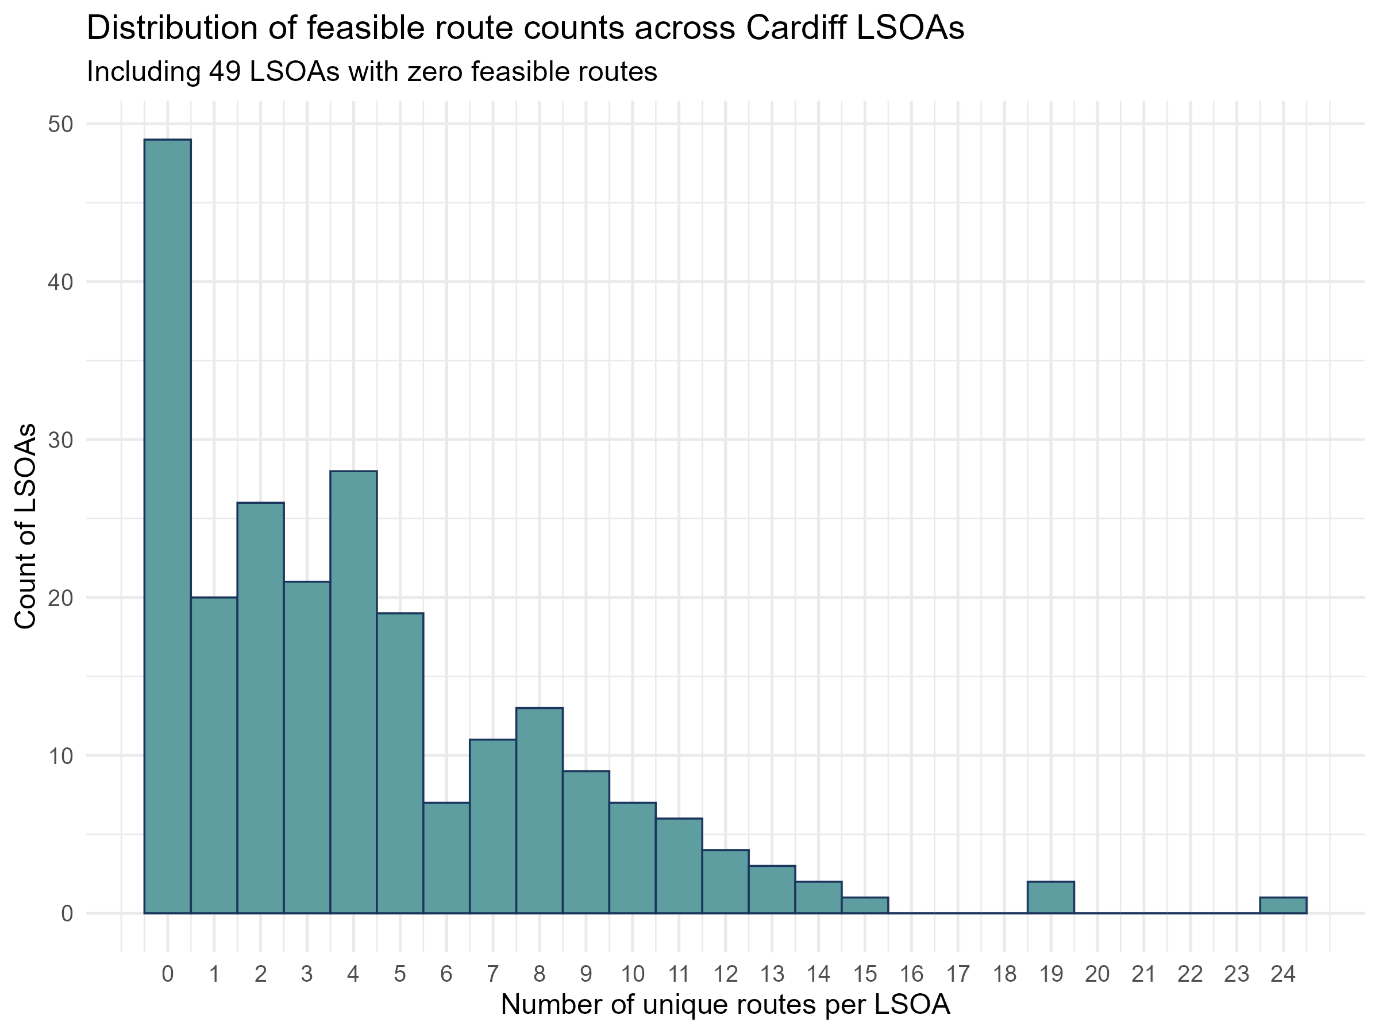
\includegraphics[width=0.85\textwidth]{figures/lsoa_route_count_distribution.png}
    \caption{Distribution of feasible public transport route counts across Cardiff LSOAs}
    \label{fig:route_count_distribution}
\end{figure}

Figure~\ref{fig:route_count_distribution} shows the distribution of feasible public transport route counts across Cardiff LSOAs. The right-skewed pattern indicates that most LSOAs have a relatively small number of feasible route options, while a smaller number of areas have substantially higher route availability. This supports the use of a route-based accessibility measure rather than relying only on simple service counts.

\subsection{Validation of top-three route temporal variability}

\begin{table}[H]
\centering
\caption{Validation of top-three route temporal variability measure}
\label{tab:top3_sd_validation}
\begin{tabular}{lcccc}
\toprule
Campus & All-route mean SD & Top-three mean SD & Absolute difference & Percentage difference \\
\midrule
Cathays & 2.76 & 2.65 & 0.11 & 3.94\% \\
Heath & 6.05 & 6.38 & 0.33 & 5.55\% \\
\bottomrule
\end{tabular}
\end{table}

Table~\ref{tab:top3_sd_validation} compares the mean temporal standard deviation from the final top-three route measure with the corresponding mean standard deviation calculated across all feasible routes. The percentage differences are small for both campuses, indicating that the top-three route formulation preserves the wider temporal variability structure of the transport network.

\subsection{Campus-level summary of top-three travel time and temporal variability}

\begin{table}[H]
\centering
\caption{Summary statistics for top-three public transport travel time and temporal variability by campus}
\label{tab:top3_time_sd_summary}
\begin{tabular}{lccccc}
\toprule
Campus & Mean time & Median time & Mean SD & Median SD & Number of LSOAs \\
\midrule
Cathays & 29.05 & 27.75 & 2.65 & 2.37 & 180 \\
Heath & 33.33 & 32.52 & 6.38 & 5.69 & 180 \\
\bottomrule
\end{tabular}
\end{table}

Table~\ref{tab:top3_time_sd_summary} provides additional campus-level summary statistics for the top-three route measure. Heath has a higher mean and median travel time than Cathays, and also a substantially higher temporal standard deviation, supporting the finding that Heath is less accessible by public transport than Cathays.
\section{Computational Implementation}
\label{app:computational_implementation}

This appendix presents selected Python code snippets from the API routing workflow. Local file paths and the API key have been omitted. The code snippets show the core implementation used to query the Google Routes API, extract journey components and construct the route-level accessibility outputs.

\subsection*{Sampled departure times and campus destinations}

\begin{lstlisting}[style=pythonappendix, caption={API endpoints, field masks and sampled departure times}, label={lst:api_setup}]
departure_times = [
    "2026-04-02T07:00:00Z",
    "2026-04-02T08:00:00Z",
    "2026-04-02T09:00:00Z",
    "2026-04-02T10:00:00Z",
    "2026-04-02T16:00:00Z",
    "2026-04-02T17:00:00Z",
    "2026-04-02T18:00:00Z",
    "2026-04-02T19:00:00Z"
]

campuses = {
    "Cathays": {"lat": 51.487207, "lon": -3.176992},
    "Heath": {"lat": 51.507156, "lon": -3.189855}
}
\end{lstlisting}

\subsection*{Origin and campus routing loop}

\begin{lstlisting}[style=pythonappendix, caption={Main loop over origin stops and campus destinations}, label={lst:origin_campus_loop}]
campus_access_rows = []

for stop_index, stop_record in enumerate(origins.to_dict("records"), start=1):
    for campus_name, campus_coords in campuses.items():
        campus_result, route_features = compute_campus_access(
            one_origin=stop_record,
            campus_name=campus_name,
            campus_lat=campus_coords["lat"],
            campus_lon=campus_coords["lon"],
            departures=departure_times
        )

        if campus_result is not None:
            campus_access_rows.append(campus_result)

    print(f"Done {stop_index}/{len(origins)}")

access_summary = pd.DataFrame(campus_access_rows)
\end{lstlisting}

\subsection*{Inner departure-time routing loop}

\begin{lstlisting}[style=pythonappendix, caption={Loop over sampled departure times for each origin--campus pair}, label={lst:departure_time_loop}]
def compute_campus_access(one_origin, campus_name, campus_lat, campus_lon, departures):
    journey_records = []
    route_json_by_departure = {}

    for departure in departures:
        matrix_result = query_matrix_once(
            one_origin["Latitude"],
            one_origin["Longitude"],
            campus_lat,
            campus_lon,
            departure
        )

        if matrix_result is None:
            continue

        route_json = query_route_detail(
            one_origin["Latitude"],
            one_origin["Longitude"],
            campus_lat,
            campus_lon,
            departure
        )

        journey_components = split_route_times(route_json)

        journey_record = {
            "departure_time": departure,
            "window": time_group(departure),
            "duration_s": matrix_result["duration_s"],
            "distance_m": matrix_result["distance_m"],

            "walk_time_min": journey_components["walk_time_min"],
            "bus_time_min": journey_components["bus_time_min"],
            "train_time_min": journey_components["train_time_min"],
            "other_transit_time_min": journey_components["other_transit_time_min"],

            "buses_used": journey_components["buses_used"],
            "trains_used": journey_components["trains_used"],
            "other_transit_legs_used": journey_components["other_transit_legs_used"],
            "transfers": journey_components["transfers"],

            "bus_routes_used": journey_components["bus_routes_used"],
            "train_lines_used": journey_components["train_lines_used"],
            "all_transit_routes_used": journey_components["all_transit_routes_used"],

            "route_json": route_json
        }

        journey_records.append(journey_record)
        route_json_by_departure[departure] = route_json

        time.sleep(0.03)

    if not journey_records:
        return None, []
\end{lstlisting}

\subsection*{Route availability and journey-time query}

\begin{lstlisting}[style=pythonappendix, caption={Matrix API query for route availability and total journey time}, label={lst:matrix_query}]
def query_matrix_once(origin_lat, origin_lon, dest_lat, dest_lon, when):
    request_body = {
        "origins": [matrix_point(origin_lat, origin_lon)],
        "destinations": [matrix_point(dest_lat, dest_lon)],
        "travelMode": "TRANSIT",
        "departureTime": when
    }

    try:
        matrix_response = requests.post(matrix_url, headers=matrix_headers, json=request_body, timeout=120)
        matrix_response.raise_for_status()
        matrix_items = matrix_response.json()
    except requests.RequestException as matrix_error:
        print("Matrix API error:", matrix_error)
        return None

    if not matrix_items:
        return None

    first_item = matrix_items[0]

    if first_item.get("condition") != "ROUTE_EXISTS":
        return None

    duration_s = secs_from_google(first_item.get("duration"))
    if duration_s is None:
        return None

    return {
        "duration_s": duration_s,
        "distance_m": first_item.get("distanceMeters")
    }
\end{lstlisting}

\subsection*{Detailed route query}

\begin{lstlisting}[style=pythonappendix, caption={Detailed route query for step-level journey information}, label={lst:route_detail_query}]
def query_route_detail(origin_lat, origin_lon, dest_lat, dest_lon, when):
    request_body = {
        "origin": route_point(origin_lat, origin_lon),
        "destination": route_point(dest_lat, dest_lon),
        "travelMode": "TRANSIT",
        "departureTime": when,
        "computeAlternativeRoutes": False
    }

    try:
        route_response = requests.post(route_url, headers=route_headers, json=request_body, timeout=120)
        route_response.raise_for_status()
        return route_response.json()
    except requests.RequestException as route_error:
        print("Route API error:", route_error)
        return None
\end{lstlisting}

\subsection*{Route decomposition into CSV variables}

\begin{lstlisting}[style=pythonappendix, caption={Decomposition of route steps into journey-time components}, label={lst:route_decomposition}]
def split_route_times(route_json):
    if route_json is None or "routes" not in route_json or len(route_json["routes"]) == 0:
        return {
            "route_detail_time_s": None,
            "route_detail_time_min": None,
            "route_detail_distance_m": None,
            "walk_time_s": None,
            "walk_time_min": None,
            "transit_time_s": None,
            "transit_time_min": None,
            "bus_time_s": None,
            "bus_time_min": None,
            "train_time_s": None,
            "train_time_min": None,
            "other_transit_time_s": None,
            "other_transit_time_min": None,
            "buses_used": None,
            "trains_used": None,
            "other_transit_legs_used": None,
            "transfers": None,
            "bus_routes_used": None,
            "train_lines_used": None,
            "all_transit_routes_used": None
        }

    first_route = route_json["routes"][0]
    collapsed_steps = collapse_consecutive_steps(route_json)

    walk_s = sum(step["duration_s"] for step in collapsed_steps if step["mode"] == "WALK")
    transit_s = sum(step["duration_s"] for step in collapsed_steps if step["mode"] == "TRANSIT")

    bus_s = sum(
        step["duration_s"]
        for step in collapsed_steps
        if step["mode"] == "TRANSIT" and step.get("transit_submode") == "BUS"
    )

    train_s = sum(
        step["duration_s"]
        for step in collapsed_steps
        if step["mode"] == "TRANSIT" and step.get("transit_submode") == "TRAIN"
    )

    other_transit_s = sum(
        step["duration_s"]
        for step in collapsed_steps
        if step["mode"] == "TRANSIT" and step.get("transit_submode") == "OTHER_TRANSIT"
    )

    bus_legs = [
        step for step in collapsed_steps
        if step["mode"] == "TRANSIT" and step.get("transit_submode") == "BUS"
    ]

    train_legs = [
        step for step in collapsed_steps
        if step["mode"] == "TRANSIT" and step.get("transit_submode") == "TRAIN"
    ]

    other_transit_legs = [
        step for step in collapsed_steps
        if step["mode"] == "TRANSIT" and step.get("transit_submode") == "OTHER_TRANSIT"
    ]

    all_transit_legs = [step for step in collapsed_steps if step["mode"] == "TRANSIT"]

    bus_routes_used = sorted({
        step.get("line_name")
        for step in bus_legs
        if step.get("line_name") and step.get("line_name") != "UNKNOWN"
    })

    train_lines_used = sorted({
        step.get("line_name")
        for step in train_legs
        if step.get("line_name") and step.get("line_name") != "UNKNOWN"
    })

    all_transit_routes_used = sorted({
        step.get("line_name")
        for step in all_transit_legs
        if step.get("line_name") and step.get("line_name") != "UNKNOWN"
    })

    total_journey_s = secs_from_google(first_route.get("duration"))

    return {
        "route_detail_time_s": total_journey_s,
        "route_detail_time_min": None if total_journey_s is None else total_journey_s / 60.0,
        "route_detail_distance_m": first_route.get("distanceMeters"),

        "walk_time_s": walk_s,
        "walk_time_min": walk_s / 60.0,

        "transit_time_s": transit_s,
        "transit_time_min": transit_s / 60.0,

        "bus_time_s": bus_s,
        "bus_time_min": bus_s / 60.0,

        "train_time_s": train_s,
        "train_time_min": train_s / 60.0,

        "other_transit_time_s": other_transit_s,
        "other_transit_time_min": other_transit_s / 60.0,

        "buses_used": len(bus_legs),
        "trains_used": len(train_legs),
        "other_transit_legs_used": len(other_transit_legs),

        "transfers": max(0, len(all_transit_legs) - 1),

        "bus_routes_used": "; ".join(bus_routes_used) if bus_routes_used else None,
        "train_lines_used": "; ".join(train_lines_used) if train_lines_used else None,
        "all_transit_routes_used": "; ".join(all_transit_routes_used) if all_transit_routes_used else None
    }
\end{lstlisting}

\subsection*{Summary construction and CSV export}

\begin{lstlisting}[style=pythonappendix, caption={Construction and export of campus-specific CSV outputs}, label={lst:csv_export}]
journey_times_df = pd.DataFrame(journey_records)

avg_duration_s = journey_times_df["duration_s"].mean()
median_duration_s = journey_times_df["duration_s"].median()

closest_to_avg_idx = (journey_times_df["duration_s"] - avg_duration_s).abs().idxmin()
representative_departure = journey_times_df.loc[closest_to_avg_idx, "departure_time"]
representative_route_json = route_json_by_departure.get(representative_departure)

summary = {
    "origin_stop_id": one_origin["stop_id"],
    "origin_stop_name": one_origin["stop_name"],
    "campus": campus_name
}

summary.update({
    "avg_total_time_s": avg_duration_s,
    "avg_total_time_min": avg_duration_s / 60.0,
    "median_total_time_s": median_duration_s,
    "median_total_time_min": median_duration_s / 60.0,
    "avg_distance_m": journey_times_df["distance_m"].mean(),
    "n_times_found": len(journey_times_df),
    "am_or_pm_average_used": "AM_and_PM",
    "am_avg_time_min": journey_times_df.loc[journey_times_df["window"] == "AM", "duration_s"].mean() / 60.0
        if (journey_times_df["window"] == "AM").any() else None,
    "pm_avg_time_min": journey_times_df.loc[journey_times_df["window"] == "PM", "duration_s"].mean() / 60.0
        if (journey_times_df["window"] == "PM").any() else None,

    "avg_walk_time_min": journey_times_df["walk_time_min"].mean(),
    "avg_bus_time_min": journey_times_df["bus_time_min"].mean(),
    "avg_train_time_min": journey_times_df["train_time_min"].mean(),
    "avg_other_transit_time_min": journey_times_df["other_transit_time_min"].mean(),

    "avg_buses_used": journey_times_df["buses_used"].mean(),
    "avg_trains_used": journey_times_df["trains_used"].mean(),
    "avg_transfers": journey_times_df["transfers"].mean(),

    "detail_route_time_used": representative_departure
})

access_summary = pd.DataFrame(campus_access_rows)

if access_summary.empty:
    print("No valid routes returned. Summary dataframe is empty.")
else:
    cathays_df = access_summary[access_summary["campus"] == "Cathays"].copy()
    heath_df = access_summary[access_summary["campus"] == "Heath"].copy()

    cathays_df.to_csv(out_cathays2, index=False)
    heath_df.to_csv(out_heath2, index=False)
    access_summary.to_csv(out_combined2, index=False)
\end{lstlisting}



\end{appendices}

\end{document}